\cleardoublepage % memastikan bab baru dimulai di halaman ganjil (kanan)
\chapter{STUDI LITERATUR}
\label{chap:studi-literatur}

% Anda dapat menambahkan pengantar umum untuk bab ini di sini jika diperlukan.
% \lipsum[1] % Contoh teks pengisi

\section{Pembelajaran Adaptif dan Asesmen Adaptif}
\label{sec:adaptive_learning_assessment}
Lingkungan pembelajaran adaptif (\textit{adaptive learning environments}) bertujuan
untuk meningkatkan perolehan pembelajaran individu dan pengalaman pemelajar dalam
lingkungan pembelajaran yang dipersonalisasi. Untuk mendukung pengembangan lingkungan
pembelajaran adaptif, diperlukan metode asesmen pengetahuan yang
adaptif untuk menilai keterampilan pemelajar \autocite{Minn2022}. Menurut \textcite{Ihichr2024}, 
penilaian pemelajar adalah salah satu momen utama dalam proses pendidikan.

% \subsection{Definisi dan Prinsip Pembelajaran Adaptif}
Pembelajaran adaptif (\textit{adaptive learning}) adalah metode pembelajaran
yang menyesuaikan dan mempersonalisasi proses pembelajaran, terutama konten pembelajarannya, agar sesuai dengan situasi dan keadaan pemelajar. Tujuan dari
\textit{adaptive learning system} (ALS) atau sistem pembelajaran adaptif
adalah untuk mengubah instruksi penyajian materi pembelajaran menggunakan seperangkat aturan yang telah
ditentukan sehingga materi pembelajaran disesuaikan dengan
kebutuhan dan perilaku pemelajar. Pembelajaran adaptif memungkinkan
pemelajar menjadi kolaborator dalam proses pendidikan, tidak hanya menjadi penerima informasi pasif. Hal ini dikarenakan setiap pemelajar memiliki jalur pembelajaran optimal tersendiri yang terdiri dari banyak titik terhubung, dengan setiap titik mewakili komponen pengetahuan atau keterampilan tertentu \autocite{Ihichr2024}.

Pembelajaran adaptif mempertimbangkan banyak aspek, seperti: tingkat kemampuan pemelajar saat ini, kebutuhan unik masing-masing pemelajar, gaya belajar masing-masing pemelajar, dan interaksi pemelajar yang berbeda-beda, untuk mengindividualisasi semua komponen proses pembelajaran. Komponen proses pembelajaran yang dapat diindividualisasikan antara lain: konten, antarmuka, gaya belajar, dan asesmen. Oleh karena itu, pembelajaran adaptif memungkinkan seorang pemelajar untuk berkembang ke pembelajaran yang lebih menantang berdasarkan kinerjanya, sambil tetap memberikan dukungan kepada pemelajar lainnya untuk menguasai keterampilan tertentu. Pendekatan ini memastikan bahwa pemelajar tidak dibatasi
oleh kecepatan kelas tetapi dapat mengikuti kecepatan belajar mereka sendiri.
Dengan demikian, pengajar dan pemelajar sama-sama dapat membuat keputusan yang tepat pada saat yang tepat, dengan mengikuti kurva belajar dan lintasan belajar (\textit{learning path}). Singkatnya, pembelajaran adaptif berusaha untuk menyesuaikan pengalaman pembelajaran untuk membantu pemelajar mencapai tujuan pembelajaran mereka dengan meniru interaksi personal antara seorang pengajar dan
seorang pemelajar \autocite{Ihichr2024}.

% \subsection{Peran Asesmen Adaptif}
Pernyataan oleh psikolog Lauren Resnick, "Apa yang kita nilai adalah apa yang kita hargai. Kita akan mendapatkan (hasil dari) apa yang kita nilai, dan jika kita tidak menilainya, kita tidak mendapatkannya", menunjukkan pentingnya asesmen sebagai langkah utama dan kritis dalam proses pendidikan. Banyak sistem pembelajaran adaptif lebih fokus
pada asesmen daripada konten. Data asesmen yang dikumpulkan dari respons pemelajar digunakan untuk mempersonalisasi proses pembelajaran, menciptakan jalur yang disesuaikan berdasarkan hasil. Jalur ini terus diperbarui dengan setiap asesmen.
Dengan demikian, asesmen pemelajar dianggap sebagai faktor krusial untuk proses pembelajaran yang sukses \autocite{Ihichr2024}.

Menurut \textcite{Ihichr2024} asesmen adaptif memungkinkan pemilihan pertanyaan berdasarkan kinerja peserta
ujian, berbeda dengan pengujian konvensional yang setiap \textit{item} dalam pengujian sudah tetap dan pasti dihadapi setiap peserta ujian terlepas dari tingkat pengetahuan mereka. Asesmen adaptif menyediakan tes
singkat yang dipersonalisasi, \textit{item}-nya berubah tergantung pada respons
pemelajar, dan kesulitan setiap pertanyaan berkorelasi dengan jawaban pertanyaan
sebelumnya. Singkatnya, asesmen adaptif berusaha menghindari penyajian pertanyaan
mudah kepada pemelajar yang mahir dan
pertanyaan menantang tidak disajikan kepada pemelajar yang mengalami kesulitan. Pendapat lain dari \textcite{Halkiopoulos2024} menambahkan penjelasan bahwa sistem asesmen adaptif adalah sistem yang secara terus-menerus menyesuaikan proses asesmennya berdasarkan tingkat kesulitan, kinerja, preferensi, motivasi, pengetahuan, dan tujuan pembelajaran yang ditunjukkan oleh pemelajar.

\subsection{Jenis Penilaian}
Menurut \textcite{Ihichr2024}, asesmen pengetahuan secara global dapat dibagi menjadi
tiga jenis: sumatif, formatif, dan praasesmen. Umumnya, asesmen sumatif lebih
dominan daripada asesmen formatif dalam \textit{e-learning}, tetapi dua jenis
terakhir telah menunjukkan potensi lebih, terutama dalam pembelajaran adaptif.


\begin{enumerate}
    % \subsubsection{Asesmen Sumatif}
    \item Asesmen sumatif juga dikenal sebagai asesmen pembelajaran (\textit{assessment of
    learning}). Jenis evaluasi ini terjadi di akhir pembelajaran untuk mengukur
    pencapaian pemelajar dan memverifikasi penguasaan kurikulum. Asesmen ini
    bertujuan menilai kemajuan kumulatif pemelajar \autocite{Ihichr2024}. Informasi
    dari asesmen sumatif dapat digunakan secara formatif untuk memandu aktivitas
    mereka di pembelajaran selanjutnya \autocite{Minn2022}.

    % \subsubsection{Asesmen Formatif}
    \item Asesmen formatif atau yang disebut juga asesmen pembelajaran \linebreak
    (\textit{assessment for learning}) terjadi sepanjang siklus pembelajaran
    untuk memberikan informasi umpan balik kepada pengajar dan pemelajar sehingga membantu
    meningkatkan pengalaman belajar mereka. Jenis asesmen ini menilai kualitas
    pembelajaran dengan memposisikan asesmen antara proses mengajar dan proses belajar, alih-alih diposisikan hanya di akhir proses pembelajaran. Ketika asesmen
    formatif sangat tertanam dalam lingkungan pembelajaran hingga pemisahan antara
    asesmen dan pembelajaran benar-benar sulit dibedakan, konsep
    ini dikenal sebagai \textit{stealth assessment}. Asesmen formatif memungkinkan sistem
    untuk menyempurnakan lintasan pembelajaran, meningkatkan keterlibatan dan antusiasme
    pemelajar, serta mengembangkan disiplin \autocite{Ihichr2024}.
    
    % \subsubsection{Pra-Asesmen}
    \item Praasesmen atau yang dikenal juga sebagai asesmen diagnostik adalah asesmen yang mengukur kompetensi awal setiap pemelajar. Ini dilakukan untuk memberikan gambaran yang jelas kepada
    pengajar tentang tingkat keterampilan pemelajar. Praasesmen biasanya dilakukan di awal pembelajaran dan dirancang
    untuk mengukur pengetahuan yang sudah diperoleh sebelumnya oleh pemelajar sehingga bisa
    mengidentifikasi kebutuhan, kompetensi, dan pengetahuan sebelumnya
    dari pemelajar tersebut. Identifikasi ini selanjutnya bisa membantu mengarahkan pemelajar ke kurikulum yang paling sesuai
    \autocite{Ihichr2024}.
\end{enumerate}

\subsection{Luaran yang Dinilai}
\textcite{Wei2021} sebagaimana dikutip dalam \textcite{Ihichr2024} mendefinisikan tiga hasil pembelajaran utama yang dinilai
dalam pembelajaran, yaitu hasil pembelajaran kognitif, perilaku, dan afektif.
Studi tersebut menunjukkan bahwa ketiga aspek ini saling berkorelasi.

\begin{enumerate}
    % \subsubsection{Luaran Kognitif}
    \item \textbf{Luaran Kognitif:} luaran ini secara mendasar berkaitan dengan pengetahuan yang diperoleh dan
    keterampilan intelektual. Pengetahuan adalah semua informasi yang telah dipelajari
    pemelajar dari suatu topik, tetapi keterampilan intelektual menyangkut kemampuan yang
    berbeda, seperti penalaran, proses berpikir, dan pengambilan keputusan.

    % \subsubsection{Luaran Perilaku}
    \item \textbf{Luaran Perilaku:} luaran perilaku merujuk pada pengukuran keterlibatan pemelajar dengan memantau
    perilakunya selama pembelajaran seperti durasi dan waktu belajar, partisipasi dalam
    forum dan diskusi, pengumpulan tugas, dan penyelesaian tes.

    % \subsubsection{Luaran Afektif}
    \item \textbf{Luaran Afektif:} luaran ketiga ini berkaitan dengan persepsi pemelajar, kepuasan mereka terhadap pembelajaran,
    apresiasi terhadap pengalaman belajar mereka, dan manfaat yang diharapkan oleh mereka
    ketika mendaftarkan diri mengikuti suatu pembelajaran. Sebagian besar pembelajaran dan
    asesmen di pendidikan tinggi berkonsentrasi pada hasil kognitif daripada hasil afektif
    dan perilaku.
\end{enumerate}

\subsection{Taksonomi Bloom dalam Asesmen Kognitif}
Kerangka kerja fundamental yang digunakan untuk mengklasifikasikan tujuan pendidikan dan mengukur kedalaman kognitif pemelajar adalah \textit{Bloom's Revised Taxonomy}. Sebagaimana dijelaskan oleh \textcite{Gosselin2018}, taksonomi ini membagi domain kognitif menjadi enam tingkatan hierarkis, yang bergerak dari proses berpikir tingkat rendah (\textit{lower-order cognition}) menuju tingkat tinggi (\textit{high-level cognition}). Tingkatan tersebut dimulai dari \textit{Remembering} (mengingat) dan \textit{Understanding} (memahami) sebagai fondasi dasar, kemudian berlanjut ke \textit{Applying} (menerapkan), \textit{Analyzing} (menganalisis), \textit{Evaluating} (mengevaluasi), hingga puncaknya pada \textit{Creating} (mencipta). Dalam konteks asesmen, idealnya \textit{Performance Indicators} (PI) dirancang dengan memadukan berbagai level ini sehingga pemelajar tidak hanya dituntut untuk mengingat fakta, tetapi juga menerapkan materi yang dipelajari dalam cara-cara yang kompleks. Penggunaan taksonomi ini memungkinkan penerjemahan luaran pembelajaran yang abstrak menjadi perilaku yang dapat diamati (\textit{observable behaviors}) dan diukur secara konkret.

Penerapan taksonomi ini dalam sistem asesmen memerlukan instrumen yang presisi, seperti penggunaan \textit{descriptive rubrics} (rubrik deskriptif). \textcite{Gosselin2018} menekankan bahwa penggunaan rubrik deskriptif yang diselaraskan dengan kata kerja operasional Bloom dapat meningkatkan konsistensi penilaian antarevaluator dan memberikan umpan balik yang lebih bermakna dibandingkan sekadar skala numerik. Rubrik ini mendeskripsikan variasi tingkat kinerja untuk setiap kriteria secara spesifik. Misalnya dalam menilai kemampuan desain teknik, indikator kinerja dapat berupa kemampuan membuat asumsi penyederhanaan dan mengevaluasi solusi (\textit{Evaluating}). Pendekatan ini juga relevan untuk asesmen sejawat (\textit{peer assessment}) karena rubrik yang terstruktur digunakan dalam asesmen untuk membantu pemelajar menilai kontribusi rekannya secara objektif berdasarkan deskripsi kinerja yang jelas, bukan sekadar persepsi subjektif.

Dalam disiplin ilmu komputasi, penggunaan kata kerja standard Bloom sering kali tidak memadai untuk menangkap nuansa teknis dari tugas-tugas pemrograman dan sistem informasi. Untuk mengatasi keterbatasan ini, \textcite{ACM2023} melalui \textit{ACM Committee for Computing Education in Community Colleges} (CCECC) mengusulkan peningkatan taksonomi dengan menambahkan 56 kata kerja spesifik komputasi yang mereka sebut dengan istilah \textit{enhanced verbs}. Modifikasi ini memetakan aktivitas teknis ke dalam level kognitif yang sesuai. Sebagai contoh, aktivitas \textit{Code} (mengodekan), \textit{Build} (membangun), dan \textit{Decrypt} (mendekripsi) dikategorikan ke dalam level \textit{Applying}. Sementara itu, aktivitas yang membutuhkan pemecahan masalah lebih dalam seperti \textit{Debug} (men-debug), \textit{Optimize} (mengoptimalkan), dan \textit{Refactor} diposisikan pada level \textit{Evaluating}. Aktivitas sintesis seperti \textit{Script} (membuat skrip), \textit{Virtualize} (memvirtualisasi), dan \textit{Program} (membuat program solusi) ditempatkan pada level tertinggi, yaitu \textit{Creating}.

Integrasi kata kerja komputasi ini memungkinkan perancangan kompetensi-kompetensi yang lebih akurat. Kompetensi yang mengintegrasikan pengetahuan (\textit{knowledge}), keterampilan (\textit{skills}), dan disposisi (\textit{dispositions}) dalam konteks tertentu \autocite{ACM2023}. Dalam lingkungan pembelajaran adaptif, pemetaan ini krusial untuk melacak kemajuan pemelajar. Seorang pemelajar mungkin memulai pembelajaran pada level \textit{Applying} dengan menerjemahkan spesifikasi menjadi kode, namun seiring waktu diharapkan berkembang ke level \textit{Creating} dengan mengimplementasikan solusi untuk masalah abstrak. \textcite{ACM2023} juga menyoroti bahwa disposisi atau aspek sikap (seperti \textit{collaborative} dan \textit{meticulous}) dapat dikaitkan dengan kompetensi teknis yang dikembangkan tersebut. Dengan demikian, sistem asesmen tidak hanya melacak kebenaran sintaksis kode, tetapi juga kedalaman pemahaman konseptual dan kemampuan kolaboratif pemelajar berdasarkan hierarki kognitif yang terstandardisasi.

\section{Pemodelan pemelajar (\textit{Student Modeling})}
\label{sec:student_modeling}

\textcite{Brusilovsky2016} menyatakan dalam konteks lingkungan pembelajaran adaptif, asesmen pengetahuan diperlukan
untuk membangun sebuah \textbf{\textit{student model}} (model pemelajar). Model
pemelajar adalah inti dari setiap sistem pendidikan adaptif, yang juga dikenal
sebagai \textit{learner model}. Model ini berfungsi
sebagai blok pembangunan fundamental (\textit{fundamental building block}) dari
asesmen pengetahuan \autocite{Minn2022}. Tujuan utamanya adalah untuk
merepresentasikan keadaan pengetahuan domain (\textit{domain knowledge})
pemelajar saat ini. Selain pengetahuan, \textit{student model} juga dapat
merepresentasikan informasi lain tentang pemelajar seperti tujuan pembelajaran
(\textit{learning goals}), sifat-sifat personal (\textit{personal traits}),
dan/atau preferensi. Dengan menggunakan
\textit{student model} inilah sebuah sistem adaptif dapat menyediakan berbagai
intervensi pembelajaran yang dipersonalisasi, seperti
\textit{mastery learning} atau \textit{adaptive sequencing}
(pengurutan adaptif) \autocite{Brusilovsky2016}.

Menurut \textcite{Minn2022} untuk membangun \textit{student model} secara efektif, diperlukan sebuah
\textit{domain model} (model domain) sebagai landasan.
\textit{Domain model} ini berfungsi untuk mengekstrak
\textit{\textbf{Knowledge Components}} (KCs) atau keterampilan (\textit{skills})
dan atribut laten (\textit{latent attributes}) yang mendasari setiap tugas atau
materi pembelajaran. \textit{Knowledge Components} ini adalah
faktor laten (\textit{latent factors}) yang tidak pernah dapat diamati secara
langsung, namun keberadaannya menentukan hasil atau kinerja pemelajar pada
suatu tugas. Dalam psikometri,
pemetaan antara \textit{item} (pertanyaan) dan KCs yang diperlukannya direpresentasikan dalam sebuah \textit{\textbf{Q-matrix}}.
Oleh karena itu, berbagai teknik asesmen adaptif pada dasarnya adalah algoritma yang digunakan untuk memperkirakan penguasaan
pemelajar atas KCs.

Dalam sebagian besar sistem pembelajaran terpersonalisasi,
\textit{student model} bersifat tersembunyi atau tidak dapat diamati
(\textit{unobservable}) oleh pemelajar, dan hanya digunakan oleh sistem untuk
menggerakkan adaptasi. Namun, sebuah pendekatan yang
dikenal sebagai \textbf{\textit{Open Student Modeling}} (OSM) atau
Pemodelan pemelajar Terbuka, berusaha membuat terobosan baru dengan secara sengaja
memperlihatkan aspek-aspek model tersebut kepada pemelajar. Tujuan dari
pendekatan OSM adalah untuk meningkatkan refleksi diri, pembelajaran mandiri, transparansi personalisasi, dan motivasi bagi pemelajar
\autocite{Brusilovsky2016, Ihichr2024}.

Sebuah perluasan yang lebih baru dan relevan dengan penelitian OSM adalah
\textbf{\textit{Open Social Student Modeling}} (OSSM) atau
Pemodelan pemelajar Sosial Terbuka. Ide dari OSSM adalah untuk
melengkapi aspek kognitif OSM dengan aspek sosial.
Hal ini dicapai dengan memungkinkan pemelajar mengeksplorasi model-model
rekan pemelajar dan/atau model kelas yang diagregasi. Pendekatan ini memiliki kesamaan dengan teknik \textit{gamification} seperti \textit{leaderboards} (papan peringkat), yang bertujuan memanfaatkan perbandingan sosial untuk meningkatkan motivasi dan keterlibatan pemelajar. Penelitian telah menunjukkan bahwa antarmuka OSSM, seperti yang diimplementasikan dalam \textit{MasteryGrids},
dapat meningkatkan pembelajaran, terutama untuk pemelajar dengan pengetahuan awal
yang lebih rendah \autocite{Brusilovsky2016}.

\section{Teknik dan Algoritma \textit{Adaptive Assessment}}
\label{sec:teknik_algoritma_aa}
Dalam rangka mencapai adaptivitas, sistem pembelajaran perlu memperkirakan tingkat 
kompetensi pemelajar dan tingkat kesulitan konten pembelajaran \autocite{Vesin2022}.
Berbagai teknik dan algoritma telah dikembangkan untuk memungkinkan asesmen adaptif, 
masing-masing dengan dasar teoretis dan karakteristiknya sendiri. Bagian ini mengulas
beberapa pendekatan utama yang digunakan dalam asesmen adaptif, dengan fokus pada 
\textit{Item Response Theory} (IRT), IRT* atau \textit{Bayesian IRT},
\textit{Factor Analysis} (FA), \textit{Bayesian Knowledge Tracing} (BKT),
\textit{Deep Knowledge Tracing} (DKT), dan sistem \textit{Elo rating}.

\subsection{\textit{Item Response Theory} (IRT)}
\textit{Item Response Theory (IRT)} adalah salah satu teori yang paling banyak
digunakan dalam asesmen adaptif, dengan asal-usulnya berasal dari Rasch dan Lord 
pada tahun 1950-an. Teori psikometri ini digunakan untuk memperkirakan pengetahuan 
pemelajar, mengembangkan pengukuran kognitif atau non-kognitif pemelajar, memilih 
pertanyaan berikutnya yang sesuai pada setiap momen, dan memutuskan kapan tes selesai 
\autocite{Ihichr2024}. Dalam IRT, probabilitas keberhasilan pada suatu tugas 
(\textit{item}) dipetakan sebagai fungsi dari tingkat kemahiran (\textit{ability}) 
yang mempertimbangkan keseluruhan tugas, dengan asumsi bahwa keadaan pengetahuan 
pemelajar statis selama ujian. Keadaan pengetahuan pemelajar $\theta$ dinilai berdasarkan
kemahirannya saat tes dilakukan, dan setiap \textit{item} yang diuji membantu
memberikan informasi untuk menyempurnakan estimasi keadaan pengetahuan $\theta_{i}$. 
Model IRT dasar mengasumsikan satu keterampilan tunggal dan bahwa \textit{item} 
tes bersifat unidimensional \autocite{Minn2022}. Secara formal, model IRT dasar
bisa diekspresikan dengan rumus matematika seperti berikut ini.

\begin{align}
P_{ij} &= \sigma(\theta_i - \beta_j) \notag \\
     &= \frac{1}{1 + e^{\theta_i - \beta_j}} \label{eq:rumus_irt}
\end{align}
\eqcaption{Probabilitas Keberhasilan Model IRT}

% Model IRT bisa dirancang dengan berbagai variasi parameter logistik.
% Model IRT dengan 1-Parameter Logistik 
% (1PL) hanya melibatkan satu karakteristik \textit{item}, yaitu kesulitan 
% \textit{item} (b), sedangkan model 2PL melibatkan kesulitan \textit{item} (b) 
% dan diskriminasi \textit{item} (a), dan model 3PL menambahkan karakteristik 
% ketiga, yaitu tebakan (\textit{lower asymptote}) \textit{item} (c) 
% \autocite{Handayani2025}.

Namun ada satu hal yang perlu diperhatikan, menurut \textcite{Minn2022} IRT bukanlah pendekatan \textit{Knowledge Tracing} 
karena mengasumsikan pemelajar tidak belajar selama proses pengujian sehingga lebih sesuai dianggal sebagai pendekatan \textit{Knowledge Assessment}.
Kelemahan IRT menurut \textcite{Vesin2022} adalah dalam hal kalibrasi pada sampel besar dan sulitnya melakukan komputasi untuk pembaruan yang sering karena estimasi baru terhadap keterampilan harus dihitung untuk setiap pemelajar setelah satu respons untuk satu tugas.

% \subsection{Model IRT* (\textit{Bayesian IRT})}
Selain pendekatan standard, model IRT juga dapat diterapkan dalam
kerangka kerja Bayesian, pendekatan ini
dalam \textcite{Minn2022} disebut sebagai IRT*. Pendekatan Bayesian untuk IRT
memungkinkan peneliti untuk memasukkan informasi sebelumnya
(\textit{prior information}) tentang parameter model. \textit{Prior} ini
dapat ditentukan dengan berbagai cara, seperti menggunakan estimasi parameter
dari studi sebelumnya atau menggunakan \textit{prior} yang tidak informatif jika tidak ada informasi yang tersedia. Sebagai
contoh, dalam kerangka kerja ini, tingkat kesulitan sebuah \textit{item}
dapat diperkirakan dari \textit{item} lain yang serupa, atau kemampuan
pemelajar dapat diperkirakan dari kinerjanya (\textit{performance}) pada tugas-tugas
lain. Pendekatan ini memanfaatkan pendekatan Bayesian dan
melakukan regularisasi terhadap $log P_ij$ dengan menerapkan distribusi
standard \textit{normal prior} independen ke setiap $\theta_i$ dan $\beta_j$.
Dengan demikian, model ini memaksimalkan probabilitas log posterior dari {$\theta_i$, $\beta_j$}
jika diketahui data respons {r: (i, j, r, t) $\in$ D}, dengan r adalah respons biner (nilainya antara 0 dan 1),
t adalah waktu ketika respons diberikan, dan D adalah kumpulan \textit{tuple} (i, j, r, t) yang menunjukkan
semua respons yang diberikan oleh pemelajar i pada \textit{item} j pada waktu t. Dalam penelitian oleh \textcite{Minn2022},
model IRT* dapat dirumuskan sebagai berikut.

\begin{multline}
\log P(\{\theta_i\}, \{\beta_j\}|D) = \sum_{(i,j,r,t) \in D} r\log \sigma(\theta_i - \beta_j) + (1-r) \\
\log(1 - \sigma(\theta_i - \beta_j)) - \frac{1}{2}\sum_i \theta_i^2 - \frac{1}{2}\sum_j \beta_j^2 + C \label{eq:rumus_irt_star}
\end{multline}

% \subsection{\textit{Hidden Markov Models} (HMM)}
% \textit{Hidden Markov Model} (HMM) adalah model statistik yang mengasumsikan
% bahwa sistem yang dimodelkan adalah proses Markov dengan keadaan yang tidak
% teramati (\textit{hidden states}). Dalam konteks asesmen
% pengetahuan, keadaan tersembunyi adalah penguasaan pemelajar terhadap suatu
% keterampilan. HMM memiliki dua asumsi utama. Asumsi pertama adalah bahwa
% keadaan pada waktu $t$ hanya bergantung pada keadaan pada waktu $t-1$.
% Asumsi kedua adalah bahwa observasi (misalnya, jawaban pemelajar) pada waktu $t$
% hanya bergantung pada keadaan pada waktu $t$. Dalam model
% ini, keadaan pengetahuan pemelajar dimodelkan sebagai variabel laten yang bertransisi
% antar keadaan (misalnya, dari "belum dipelajari" ke "dipelajari"), dan
% probabilitas transisi ini diperbarui berdasarkan urutan kinerja pemelajar
% yang teramati \autocite{Minn2022}.

\subsection{\textit{Factor Analysis} (FA)}
% \textit{Factor Analysis} (FA) atau Analisis Faktor adalah teknik psikometri
% yang menjelaskan korelasi dari variabel-variabel yang diamati
% (\textit{observed variables}). Dalam konteks
% asesmen adaptif, FA utamanya berfungsi untuk membangun model pemelajar,
% khususnya komponen kognitif, dengan mengeksplorasi faktor-faktor yang
% memengaruhi proses pembelajaran. Faktor-faktor ini mungkin termasuk
% pengetahuan sebelumnya (\textit{prior knowledge}), kemampuan kognitif,
% dan motivasi. FA membantu dalam menentukan \textit{item}
% yang paling baik mengukur kemahiran pemelajar dan dalam menghasilkan umpan
% balik adaptif \autocite{Ihichr2024}.

\textcite{Pavlik2009} sebagaimana dikutip dalam \textcite{Minn2022} adalah yang mengusulkan ide modifikasi dari \textit{Learning Factor Analysis} (LFA) menjadi \textit{Performance Factor Analysis} (PFA). Pengubahan ini memungkinkan jejak prediksi untuk pemelajar secara individual terhadap keterampilan-keterampilan tertentu. 

\textit{Factor Analysis} atau secara spesifiknya \textit{Performance Factor Analysis} (PFA) adalah algoritma yang mengikuti pemodelan logistik untuk dapat mengukur secara sensitif terhadap suatu indikator dalam evaluasi. Teknik ini umumnya sensitif terhadap rasio jawaban benar terhadap jawaban salah dalam suatu asesmen. Sensitivitas model terhadap indikator tersebut bisa digunakan untuk mengukur kualitas pembelajaran \autocite{Ihichr2024}.

Model PFA ini memungkinkan konjungsi keterampilan dengan cara menjumlahkan kontribusi semua keterampilan yang dibutuhkan dalam suatu pengukuran kinerja. Model ini memfasilitasi pembelajaran beragam keterampilan yang pada kenyataannya kekurangan atau kelemahan dalam suatu KC bisa dikompensasi dengan keberadaan suatu KC lainnya. Model-model \textit{factor analysis} lain juga banyak dikembangkan, beberapa contohnya adalah DASH \autocite{Lindsey2014}, SPARFA \autocite{Lan2013}, \textit{Knowledge Tracing Machines} \autocite{Vie2018}, dan DAS3H \autocite{Choffin2019}.

\subsection{\textit{Bayesian Knowledge Tracing (BKT)}}
% \textit{Hidden Markov Model} (HMM) adalah model statistik yang mengasumsikan
% bahwa sistem yang dimodelkan adalah proses Markov dengan keadaan yang tidak
% teramati (\textit{hidden states}). Dalam konteks asesmen
% pengetahuan, keadaan tersembunyi adalah penguasaan pemelajar terhadap suatu
% keterampilan. HMM memiliki dua asumsi utama. Asumsi pertama adalah bahwa
% keadaan pada waktu $t$ hanya bergantung pada keadaan pada waktu $t-1$.
% Asumsi kedua adalah bahwa observasi (misalnya jawaban pemelajar) pada waktu $t$
% hanya bergantung pada keadaan pada waktu $t$. Dalam model
% ini, keadaan pengetahuan pemelajar dimodelkan sebagai variabel laten yang bertransisi
% antar keadaan (misalnya, dari belum dipelajari ke sudah dipelajari), dan
% probabilitas transisi ini diperbarui berdasarkan urutan kinerja pemelajar
% yang teramati \autocite{Minn2022}.

% Salah satu penerapan HMM yang paling luas dalam asesmen adaptif adalah
% \textit{Bayesian Knowledge Tracing (BKT)}, suatu pendekatan yang didasarkan pada 
% \textit{Bayesian Networks} (BNs). Pendekatan ini mencoba memodelkan keterampilan 
% pemelajar dengan menghitung probabilitas penguasaan keterampilan berdasarkan 
% seperangkat parameter: menebak (\textit{guessing}), terpeleset (\textit{slipping}), 
% probabilitas bahwa keterampilan sudah dikuasai sebelumnya, dan probabilitas bahwa 
% keterampilan akan dipelajari. BKT memperhitungkan urutan waktu untuk memperkirakan 
% keterampilan baru dan mengasumsikan bahwa setiap keterampilan yang dipelajari tidak 
% pernah dilupakan \autocite{Ihichr2024}.

BKT adalah pendekatan paling awal untuk 
memodelkan keadaan pengetahuan pemelajar yang berubah dan merupakan model pertama 
yang melonggarkan asumsi keadaan pengetahuan statis. Dalam BKT standard, satu 
keterampilan diuji per \textit{item} dan keadaan penguasaan keterampilan 
pemelajar disimpulkan pada setiap waktu berdasarkan hasil sebelumnya. Pendekatan ini relevan bagi pengajar yang memanfaatkan latihan dan metode \textit{scaffolding} sebagai upaya utama dalam pembelajaran.
BKT mengandalkan model Markov untuk menyimpulkan keadaan penguasaan, dari belum dipelajari menjadi sudah dipelajari \autocite{Minn2022}. Model Markov yang digunakan dalam BKT bisa digambarkan seperti pada Gambar \ref{fig:model-standard-bkt}.

\begin{figure}[!ht]
    \centering
    \captionsetup{justification=centering}
        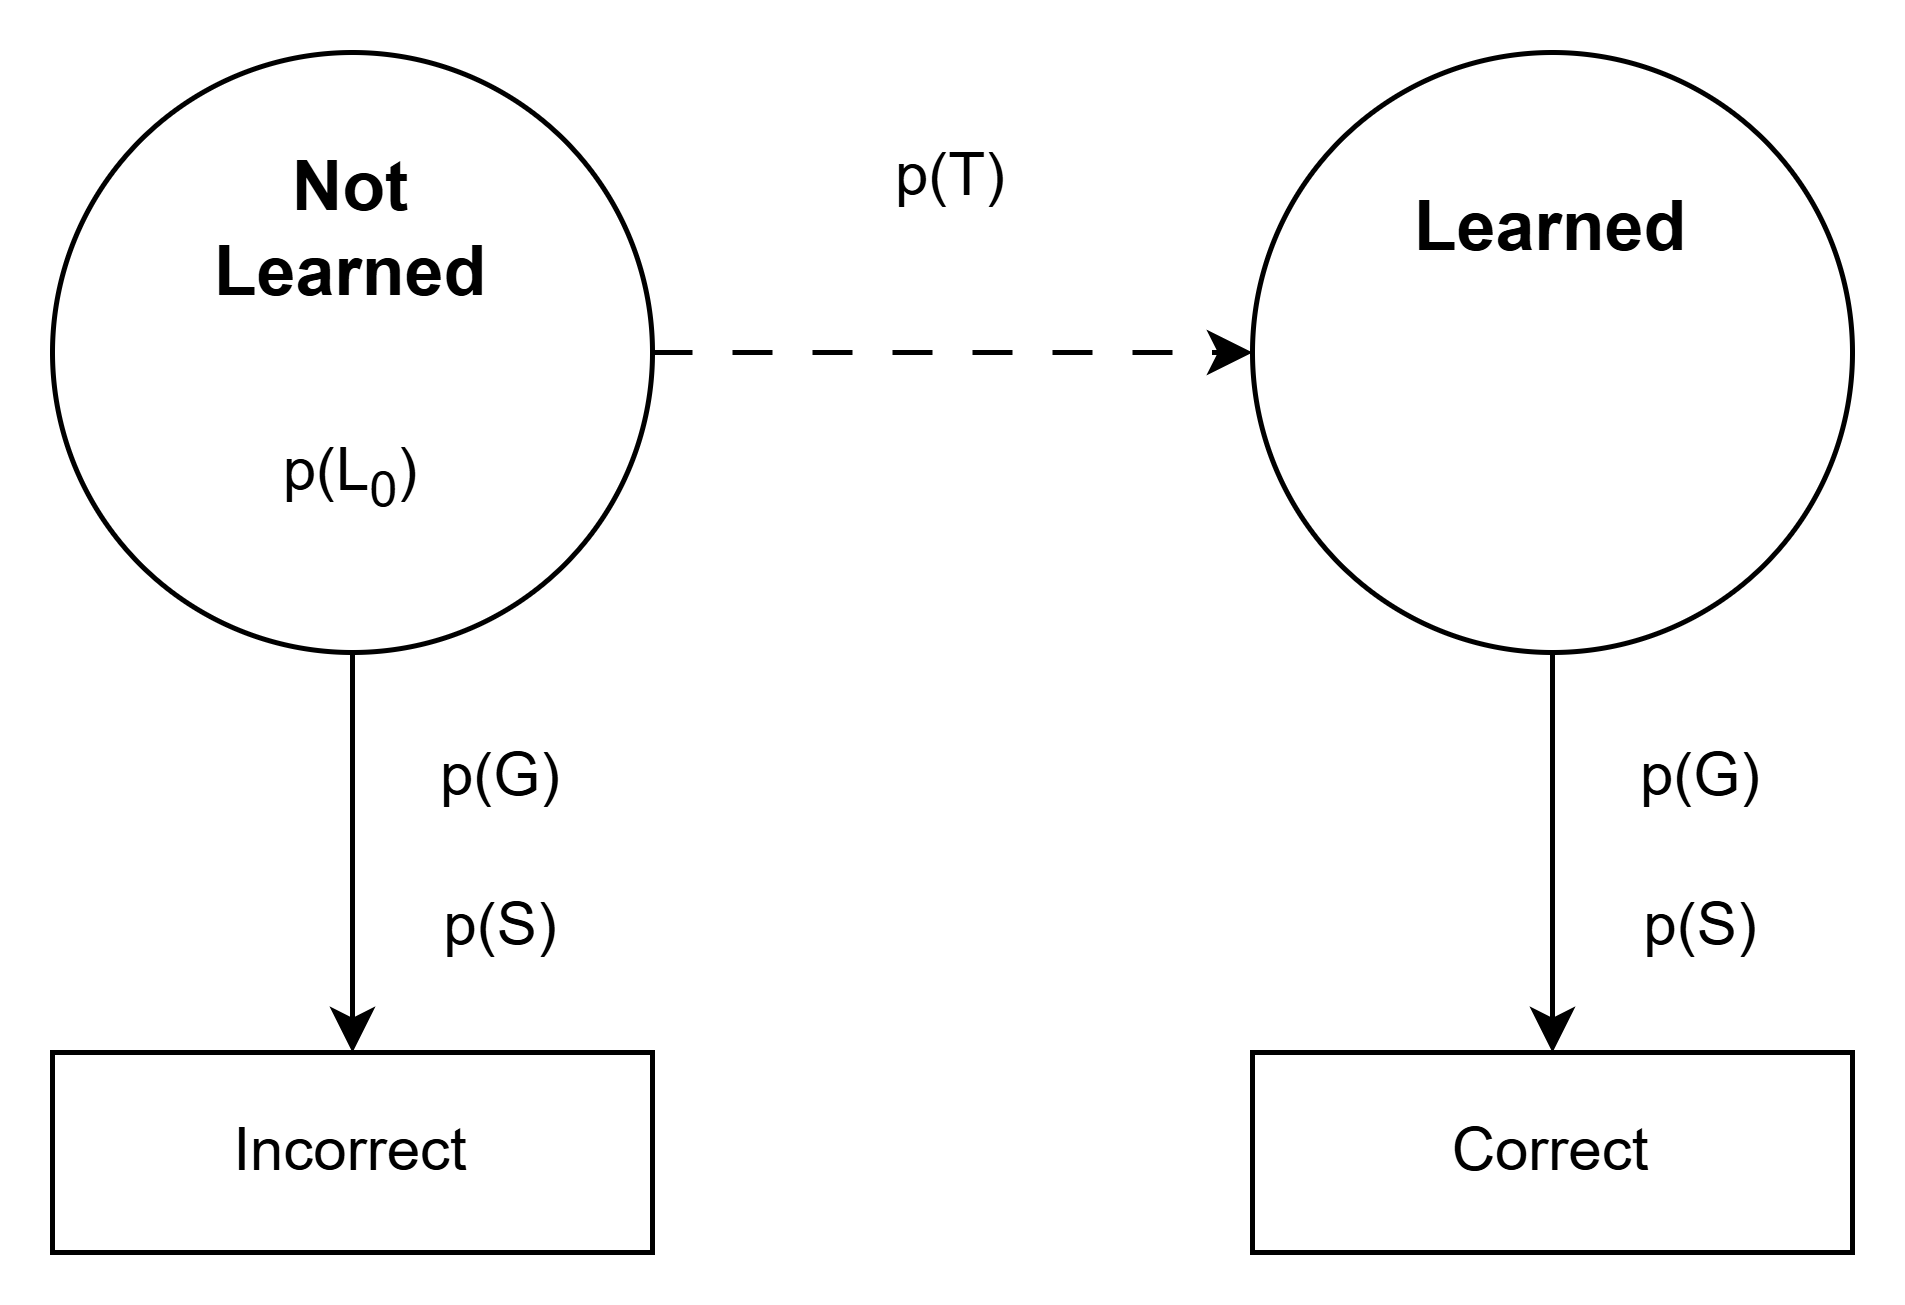
\includegraphics[width=0.75\textwidth]
        {images/standard_bkt.png}
    \caption{Contoh Model Konseptual dari BKT Standard yang Mengestimasi
    Transisi \textit{State} pemelajar dari Belum Dipelajari (\textit{Not Learned})
    menjadi Sudah Dipelajari (\textit{Learned}) (diadaptasi dari \textcite{Minn2022})}
    \label{fig:model-standard-bkt}
\end{figure}

Model standard BKT memiliki 4 parameter utama yang biasanya dipelajari dari data ketika model dibangun untuk setiap keterampilan. Probabilitas inferensial dalam model ini bergantung pada parameter yang digunakan untuk mengestimasi bagaimana pemelajar menguasai keterampilannya. Estimasi tersebut dilakukan berdasarkan rangkaian kronologis hasil biner (benar atau salah) untuk pertanyaan terkait keterampilan tersebut sejauh ini.

\subsection{\textit{Deep Knowledge Tracing (DKT)}}
\textit{Deep Knowledge Tracing (DKT)}, sebuah algoritma perintis yang
menggunakan jaringan saraf rekuren mendalam (\textit{deep recurrent neural networks})
untuk memodelkan proses pembelajaran pemelajar dan melacak pengetahuan mereka. DKT digunakan untuk
mengekstrak struktur tersembunyi antarasesmen. DKT bergantung pada model RNN dan LSTM, dua model pembelajaran mendalam yang memiliki keunggulan dalam menangkap representasi pengetahuan yang secara temporal dari rangkaian asesmen. Kemampuan ini memungkinkan kinerja 
prediksi yang jauh lebih baik di seluruh dataset asesmen historis. Selain itu,
model yang dibangun juga dapat digunakan untuk merancang asesmen berikutnya yang lebih sesuai untuk pemelajar \autocite{Ihichr2024}.

DKT menggunakan data yang diperoleh dari 
pengujian keterampilan dan hasil pengujiannya digunakan untuk memprediksi rangkaian upaya pembelajaran di masa mendatang. DKT menggunakan sejumlah besar neuron buatan 
untuk merepresentasikan keadaan pengetahuan laten dengan struktur temporal yang dinamis. Representasi ini yang memungkinkan model untuk mempelajari keadaan pengetahuan pemelajar dari data. Namun,
seperti model \textit{deep learning} lainnya, DKT sering kali berfungsi sebagai \textit{black box} dengan banyak parameter dan struktur yang kompleks sehingga sulit untuk memberikan penjelasan yang bermakna secara psikologis \autocite{Minn2022}.

\subsection{Sistem \textit{Elo rating}}
Sistem \textit{Elo rating}, yang awalnya dikembangkan untuk memberi peringkat
pemain catur, baru-baru ini digunakan dalam pendidikan untuk mengatasi beberapa
celah yang ditimbulkan oleh teknik pemodelan pemelajar yang lainnya. \textit{Elo rating} sepenuhnya bergantung
pada evaluasi kuantitatif kinerja pemelajar dan dapat memodelkan keterampilan yang
berubah seiring waktu. Ketika \textit{item} baru ditambahkan dalam sistem, tidak
perlu menetapkan kesulitan \textit{item} awal yang benar, karena sistem akan belajar
dan menetapkan tingkat kesulitan untuk konten pembelajaran berdasarkan jawaban pemelajar yang mengerjakan soal tersebut. Algoritma \textit{Elo rating} juga dapat memberikan estimasi
kesulitan tugas yang akurat dengan ukuran sampel kecil, sesuatu yang tidak mungkin
dilakukan dengan model IRT. Adaptasi \textit{Elo rating} ke
bidang pendidikan mengasumsikan bahwa pemelajar adalah pemain dan \textit{item} konten
(misalnya latihan penulisan kode program) adalah lawan \autocite{Vesin2022}.

Peringkat \textit{Elo} pemelajar
dan materi pemebalajaran diwakili oleh angka yang meningkat atau menurun tergantung pada interaksi pemelajar dengan materi pembelajaran. Perbedaan peringkat antara pemelajar dan \textit{item} pembelajaran berfungsi sebagai prediktor hasil interaksi. Algoritma \textit{Elo rating} merupakan algoritma yang hemat sumber daya komputasi, sangat sederhana untuk diimplementasikan, dan cocok untuk praktik adaptif dalam pendidikan. Implementasi
yang diusulkan oleh \textcite{Vesin2022} memperluas \textit{Elo rating} klasik dengan
mempertimbangkan parameter tambahan seperti jumlah percobaan dan waktu yang digunakan untuk memberikan adaptivitas dan
rekomendasi dalam tugas pemrograman \textit{open-ended}.

Secara spesifik, metode yang diusulkan menerapkan dua strategi, (1) memperbarui peringkat pemelajar
berdasarkan performa pemelajar pada interaksinya dengan materi pembelajaran dibandingkan nilai interaksinya dan (2)
tingkat kesulitan konten pembelajaran diperbarui berdasarkan peringkat atau skor pemelajar yang berhasil ataupun gagal dalam berhadapan dengan konten tersebut. Secara matematis, cara ini mengestimasi probabilitas seorang pemelajar \textit{i} mampu menyelesaikan latihan \textit{j} berdasarkan peringkat pemelajar saat ini dan tingkat kesulitan latihan \textit{j}.
Peringkat pemelajar dan kesulitan latihan kemudian diperbarui menurut rumus berikut,

\begin{align}
R_i &= R_{i-1} + K (W - W_e)\label{eq:rumus_elo_student}
\end{align}
\eqcaption{Perubahan Peringkat pemelajar (Ri)}
\begin{align}
D_j &= D_{j-1} + K (W_e - W)\label{eq:rumus_elo_latihan}
\end{align}
\eqcaption{Perubahan Tingkat Kesulitan Soal (Dj)}

dengan $R_i$ adalah peringkat pemelajar setelah menyelesaikan latihan ke-i,
$R_{i-1}$ adalah peringkat pemelajar sebelum menyelesaikan latihan ke-i,
$D_j$ adalah tingkat kesulitan latihan ke-j setelah pemelajar menyelesaikannya,
$D_{j-1}$ adalah tingkat kesulitan latihan ke-j sebelum pemelajar menyelesaikannya,
$K$ adalah faktor penyesuaian yang menentukan seberapa besar perubahan peringkat
atau tingkat kesulitan, nilai ini dikurangi secara bertahap seiring pemelajar menyelesaikan lebih banyak latihan,
$W$ merepresentasikan hasil dari penyelesaian latihan yang direkomendasikan (dengan kata lain adalah tingkat keberhasilan),
yang dihitung berdasarkan formula berikut.

\begin{align}
W = \left(\frac{(A_s + A_o)T_c}{2A_oT_p}\right)(a_id_i - a_it_i). \label{eq:rumus_W_elo}
\end{align}
\eqcaption{Pembobotan Skor W}

Rumus \ref{eq:rumus_W_elo} di atas adalah kunci modifikasi algoritma \textit{Elo rating} dari riset oleh \textcite{Vesin2022},
variabel-variabelnya dijelaskan dalam laporan hasil risetnya dengan definisi di bawah ini:
\begin{itemize}
    \item $A_s$: banyaknya upaya yang berhasil untuk latihan tertentu
    \item $A_o$: banyaknya total upaya untuk latihan tertentu
    \item $T_c$: banyaknya latihan yang sudah diselesaikan
    \item $T_p$: banyaknya latihan yang diselesaikan dengan benar
    \item $a_i$: bobot kepentingan kecepatan (waktu) penyelesaian
    \item $d_i$: merepresentasikan batas waktu
    \item $t_i$: merepresentasikan waktu yang dibutuhkan untuk menyelesaikan latihan
\end{itemize}

Terakhir adalah komponen $W_e$, komponen ini merepresentasikan probabilitas
seorang pemelajar mampu menyelesaikan latihan tertentu, yang dihitung berdasarkan rumus \textit{Elo} standard \autocite{Elo1978}:
\begin{align}
W_e = \frac{1}{1+10^{\frac{R_{i-1} - D_{j-1}}{400}}}. \label{eq:rumus_W_e_elo}
\end{align}
\eqcaption{Ekspektasi Keberhasilan (We)}

\subsection{Posisi Teknik dan Algoritma dalam Sistem Asesmen Adaptif Individual}
\label{ssec:arsitektur_sistem_aa_individual}
Berbagai teknik yang telah dibahas di Subbab \ref{sec:teknik_algoritma_aa} umumnya
diimplementasikan dalam sebuah siklus sistem.
Model konseptual siklus sistem yang dominan untuk asesmen adaptif
saat ini adalah siklus yang
berpusat pada pemelajar tunggal. Sebuah contoh representatif dari alur kerja ini
diimplementasikan dalam sistem ProTuS oleh \textcite{Vesin2022}, seperti yang
ditunjukkan pada Gambar \ref{fig:model-konseptual-individu}.

\begin{figure}[!ht]
    \centering
    \captionsetup{justification=centering}
        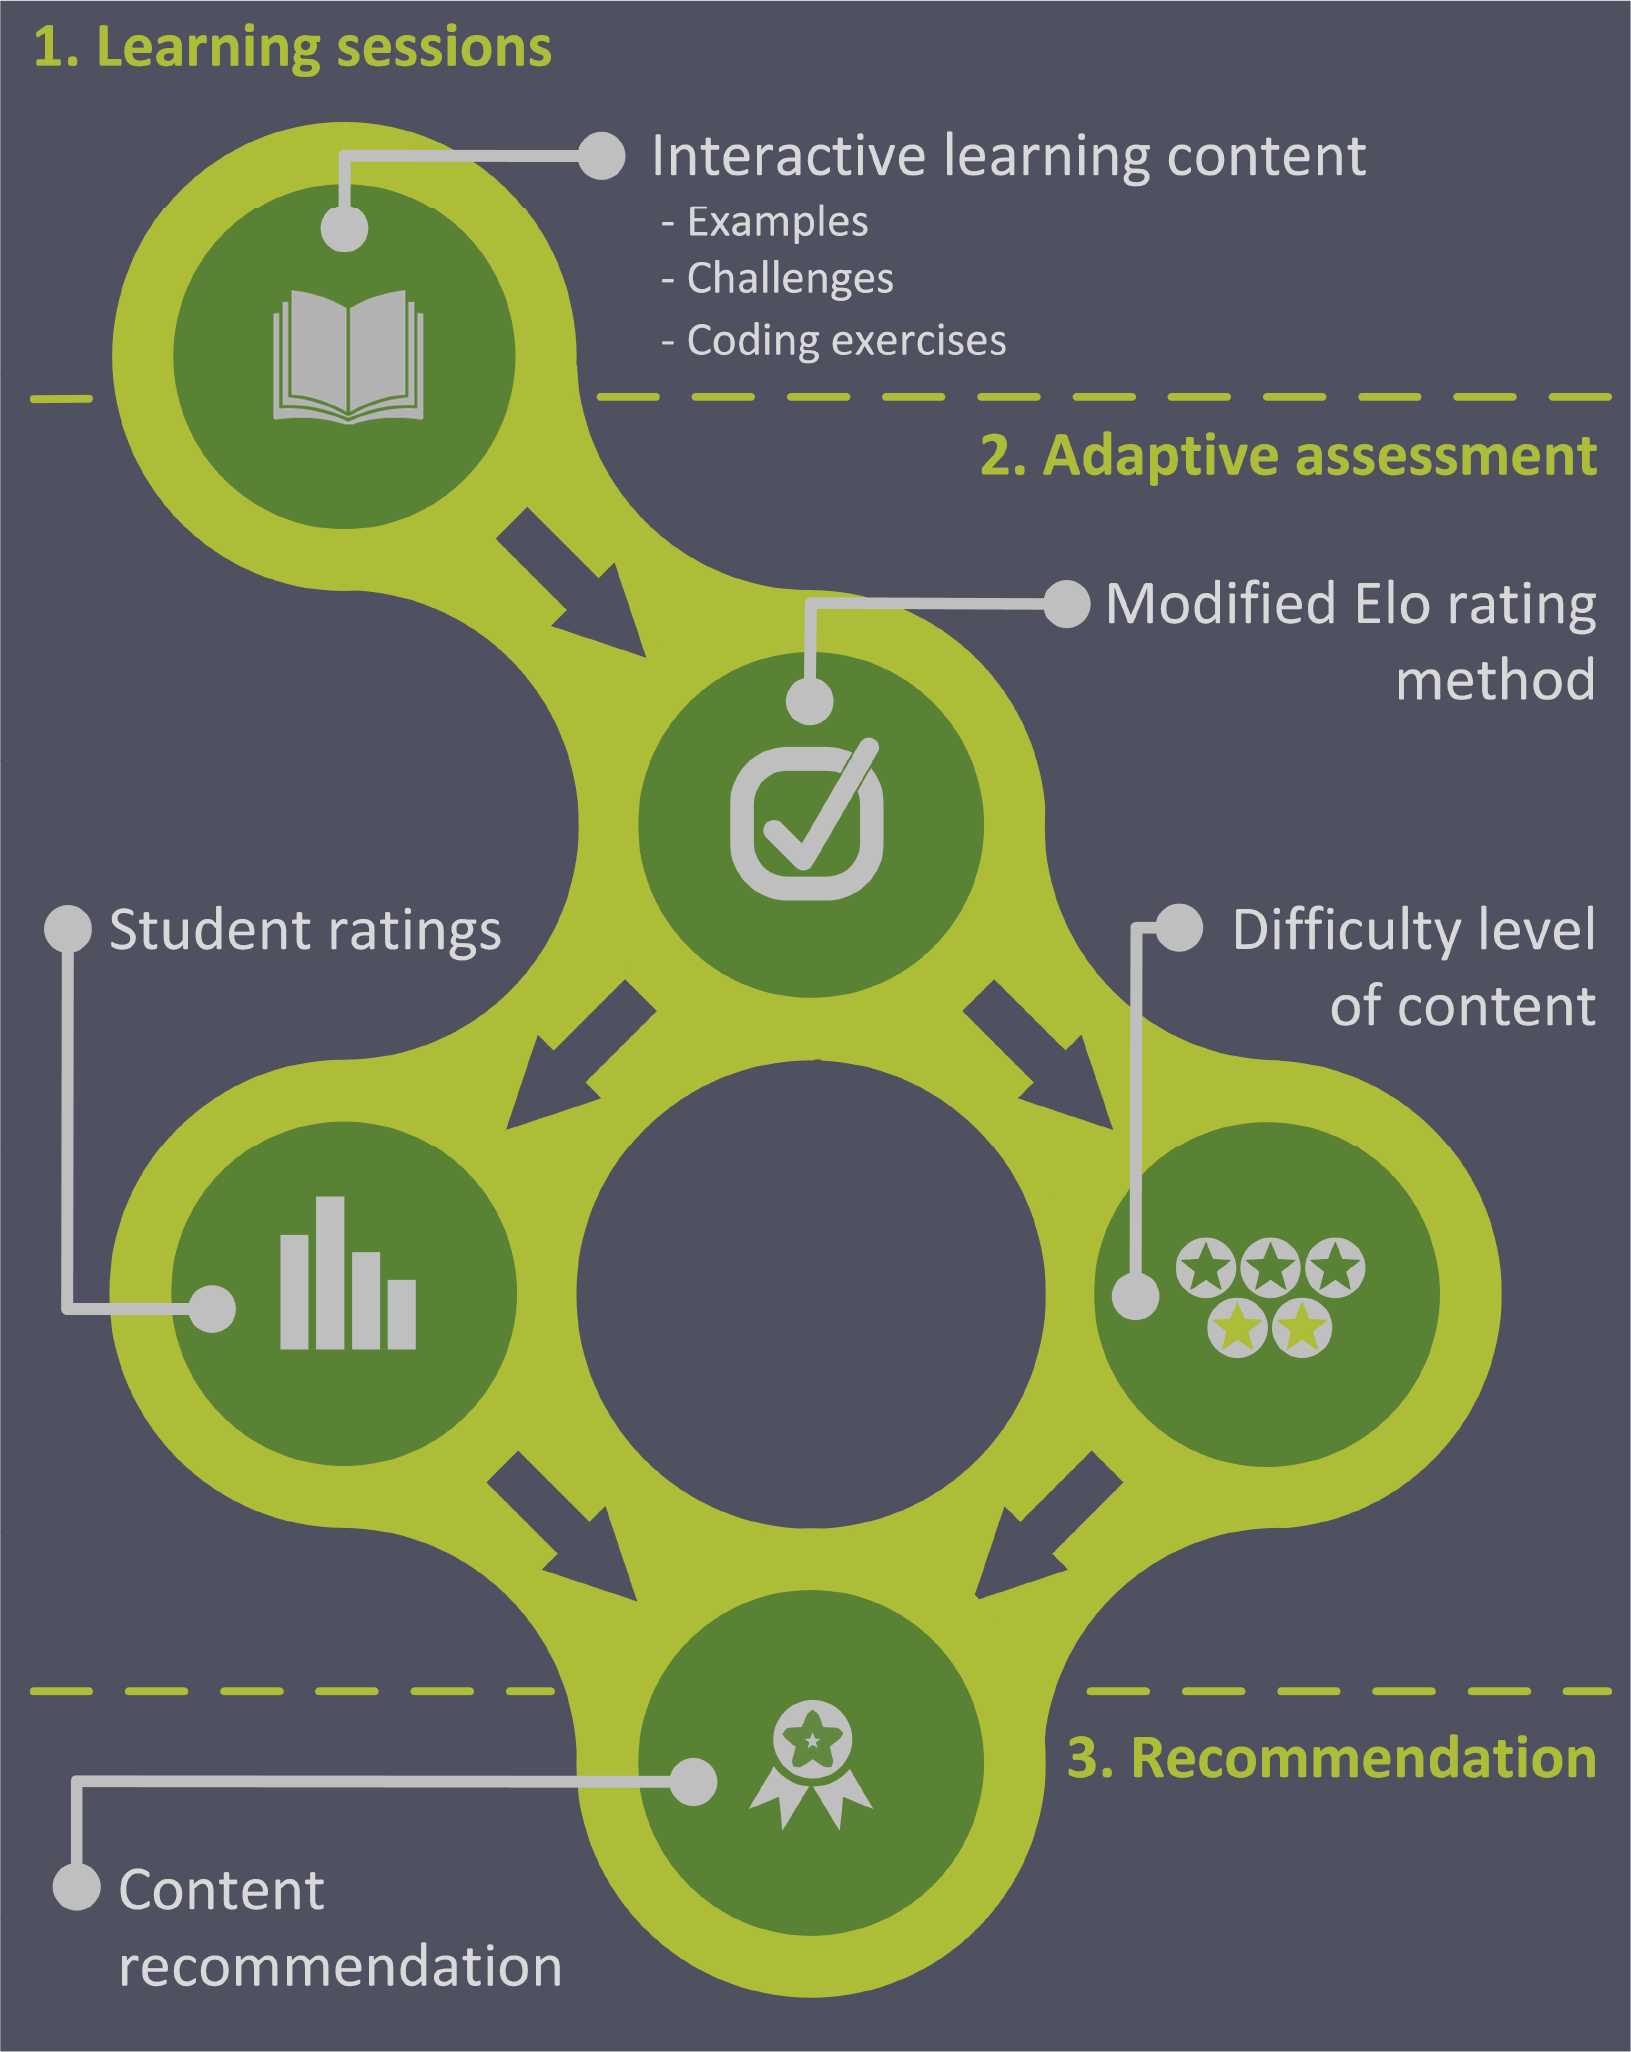
\includegraphics[width=0.8\textwidth]
        {images/vesin_fig1.png}
    \caption{Model Konseptual Alur Proses Sistem Adaptif
    Individual (dari \textcite{Vesin2022})}
    \label{fig:model-konseptual-individu}
\end{figure}

Menurut \textcite{Vesin2022} alur proses dalam model ini terdiri dari tiga tahap yang berulang:
\begin{enumerate}
    \item \textbf{Sesi Pembelajaran (\textit{Learning Sessions}):} pemelajar berinteraksi
    dengan sumber daya pembelajaran yang disediakan, seperti membaca materi
    atau menyelesaikan latihan pengodean.
    \item \textbf{Asesmen Adaptif (\textit{Adaptive Assessment}):} Saat pemelajar
    menyelesaikan aktivitas, sistem memperbarui peringkat mereka berdasarkan
    kinerja individu. Peringkat pemelajar
    (\textit{student ratings}) dan tingkat kesulitan konten
    (\textit{difficulty level of content}) dihitung menggunakan metode \textit{modified Elo rating} yang memanfaatkan rumus \ref{eq:rumus_elo_student} dan rumus \ref{eq:rumus_elo_latihan}.
    \item \textbf{Rekomendasi (\textit{Recommendation}):} Sistem kemudian 
    merekomendasikan aktivitas pembelajaran lebih lanjut yang sesuai dengan
    kemahiran pemelajar saat ini.
\end{enumerate}

Tahap modifikasi kesulitan konten pembelajaran mungkin tidak ada di semua sistem
karena beberapa teknik seperti IRT mengharuskan kesulitan konten ditetapkan sebelumnya.
Namun, secara umum akan melalui siklus seperti di atas, dan teknik serta algoritma
yang dibahas pada Subbab \ref{sec:teknik_algoritma_aa} berperan secara khusus dalam tahap asesmen adaptif.

% Masalah pada model ini adalah bahwa keseluruhan siklus bersifat individualistis.
% Algoritma asesmen (misalnya, \textit{Elo rating} yang dimodifikasi) menghitung
% keberhasilan pemelajar murni berdasarkan parameter individual, seperti
% "jumlah upaya yang berhasil/gagal", "persentase/tingkat keberhasilan
% \textit{unit test}", dan "waktu yang dibutuhkan untuk menyelesaikan latihan"
% \autocite{Vesin2022}. Model ini tidak memiliki mekanisme untuk memasukkan
% atau mengukur nilai dari interaksi sosial.

\section{\textit{Overpersonalization} dalam Konteks Pendidikan}
\label{sec:overpersonalization_dalam_pendidikan}

Implementasi algoritma personalisasi dalam sistem pembelajaran adaptif bertujuan untuk mengoptimalkan efisiensi akuisisi pengetahuan dengan menyesuaikan materi terhadap profil unik setiap pemelajar. Namun, optimasi yang terlalu agresif terhadap parameter individu tanpa mempertimbangkan aspek eksplorasi dan keberagaman informasi dapat memicu fenomena \textit{overpersonalization} \autocite{Halkiopoulos2024}. Risiko ini muncul ketika sistem menciptakan lingkungan yang terlalu tertutup, sehingga membatasi paparan pemelajar terhadap konsep-konsep baru yang krusial bagi pengembangan kognitif yang holistik. Subbab berikut akan mengulas manifestasi dari kondisi tersebut serta metrik yang digunakan untuk mengukurnya.

\subsection{Manifestasi \textit{Overpersonalization} dalam Pembelajaran}

Manifestasi dari \textit{overpersonalization} dalam lingkungan pendidikan dapat diamati melalui perubahan perilaku kognitif pemelajar saat berinteraksi dengan sistem yang terlalu terpersonalisasi. Menurut penelitian \textcite{Bahg2025}, pemelajar dalam ekosistem kognitif yang membatasi keberagaman informasi cenderung melakukan sampling informasi secara lebih selektif. Hal ini menyebabkan pembentukan representasi kategori (materi pembelajaran) yang tidak tepat karena pemelajar hanya terpapar pada subset data yang sempit dan homogen. Secara fundamental, fenomena ini mengindikasikan bahwa dampak negatif \textit{overpersonalization} tidak hanya terbatas pada isolasi informasi, tetapi juga menyebabkan distorsi pemahaman, bias dalam pengambilan sampel informasi, serta generalisasi pengetahuan yang tidak tepat \autocite{Bahg2025}. Dampak ini diperparah oleh pembentukan \textit{filter bubble} yang, sebagaimana ditunjukkan oleh \textcite{Jiang2025}, menyebabkan penurunan diversifikasi konsumsi informasi secara signifikan, yang pada akhirnya membatasi cakrawala intelektual pemelajar.

\subsection{Pengukuran \textit{Overpersonalization} dalam Pembelajaran}

Pengukuran terhadap tingkat \textit{overpersonalization} memerlukan metrik yang mampu menangkap aspek keberagaman dalam rekomendasi konten edukasi. Dalam domain sistem rekomendasi secara umum, \textcite{Ren2025} menyatakan bahwa pengukuran tingkat keberagaman dapat dilakukan menggunakan metrik variansi atau entropi, seperti \textit{Shannon Entropy}, untuk menguantifikasi seberapa luas sebaran entitas dan relasi yang dikonsumsi oleh pengguna dibandingkan dengan total ruang pengetahuan yang tersedia. Dalam konteks spesifik pembelajaran, indikasi \textit{overpersonalization} juga dapat dideteksi melalui kemunculan fenomena \textit{learning plateau} \autocite{Halkiopoulos2024}. Fenomena ini ditandai dengan stagnasi kemajuan belajar (kognitif) pemelajar yang disebabkan oleh kurangnya variasi terhadap tantangan atau tingkat kesulitan yang dihadapi. Ketika sistem terus-menerus menyajikan materi yang terlalu selaras dengan zona nyaman pemelajar tanpa memberikan paparan terhadap konsep-konsep baru yang beragam, pemelajar kehilangan stimulasi kognitif yang diperlukan untuk keluar dari stagnasi tersebut.

\section{Upaya Penyelesaian Masalah \textit{Overpersonalization} yang Ada Saat Ini}
\label{sec:upaya_penyelesaian}

Setelah memahami manifestasi kognitif dan metrik pengukuran dari \textit{overpersonalization} sebagaimana dibahas pada bagian sebelumnya, diperlukan tinjauan terhadap solusi teknis yang telah dikembangkan untuk memitigasi dampak tersebut. Masalah \textit{overpersonalization} telah menjadi perhatian utama dalam penelitian sistem rekomendasi modern karena dampaknya dalam menciptakan \textit{filter bubbles} dan \textit{echo chambers} yang menghambat pertumbuhan pengetahuan. Untuk mengatasi isolasi pengguna ini tanpa mengorbankan relevansi secara signifikan, peneliti telah mengeksplorasi berbagai pendekatan yang berusaha menyeimbangkan antara akurasi personalisasi dengan kebutuhan akan keberagaman informasi. Tiga pendekatan yang paling menonjol dan relevan melibatkan penggunaan rekomendasi berbasis kelompok (\textit{Group Recommender Systems}), pemberian kendali kepada pengguna (\textit{User Controllable Systems}), dan pemodelan komunitas secara implisit (\textit{Implicit Community Modeling}).

\subsection{Sistem Rekomendasi yang Dapat Dikontrol Pengguna (\textit{User Controllable Recommender Systems})}
\label{subsec:ucrs}

Pendekatan pertama adalah pendekatan yang dikenal sebagai \textbf{\textit{User Controllable
Recommender System}} (UCRS), pendekatan ini menerapkan sistem yang memungkinkan
pengguna memutuskan apakah ingin menghindari \textit{filter bubble} sehingga bisa memilih
\textit{bubble} mana yang akan dihindari. Secara fungsional,
\textcite{Wang2022} menjelaskan bahwa UCRS dapat memperingatkan pengguna jika
mereka terjebak dalam \textit{filter bubble}. UCRS mendukung empat jenis perintah
kontrol bagi pengguna untuk memitigasi \textit{bubble} pada dua tingkat granularitas (tingkat kedetailan) yang berbeda (\textit{fine-grained} dan \textit{coarse-grained}) dan untuk dua fitur berbeda (\textit{user} dan \textit{item}). UCRS dalam usulan \textcite{Wang2022} bisa merespons perintah-perintah kontrol tersebut untuk menyesuaikan rekomendasi secara langsung (\textit{on the
fly}). Sistem ini menyediakan perintah kontrol item, seperti perintah untuk meningkatkan item yang disukai oleh kelompok pengguna lain atau item dalam kategori target tertentu.

\begin{figure}[!ht] 
    \centering
    \captionsetup{justification=centering}
    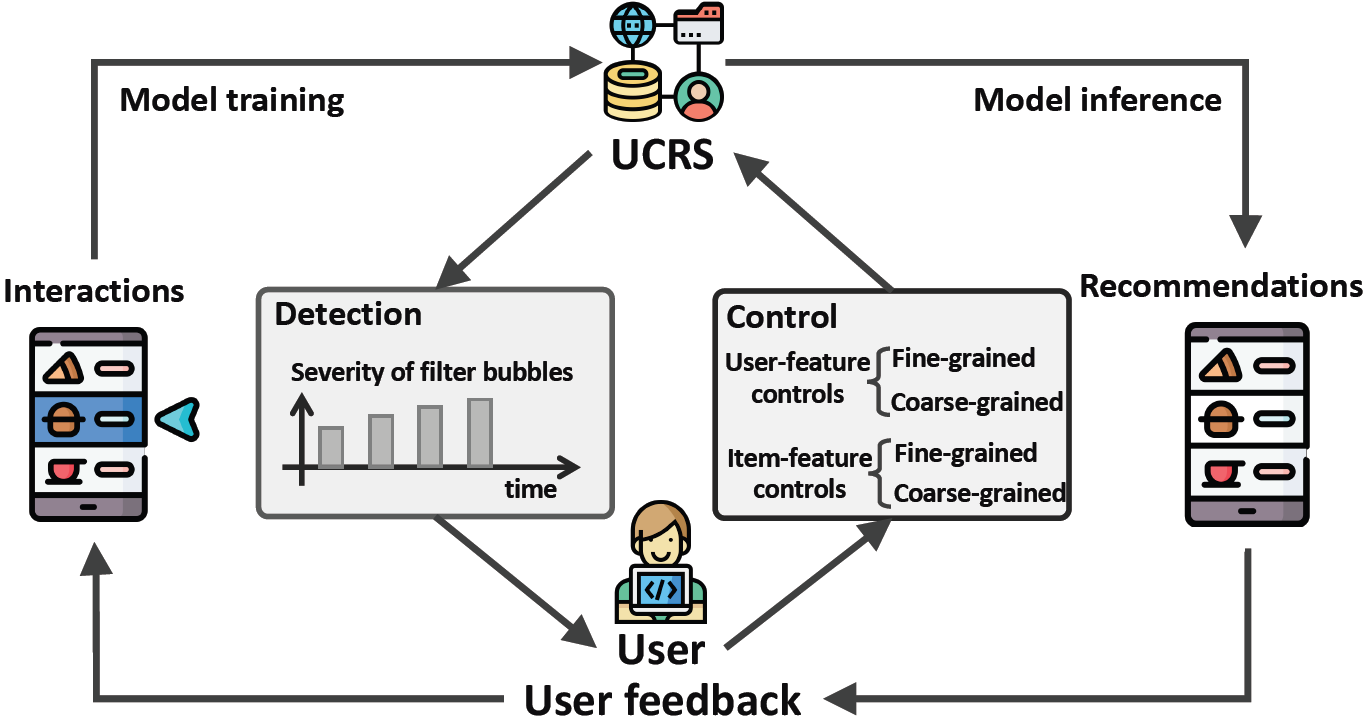
\includegraphics[width=1.0\textwidth]
    {images/UCRS_model.png}
    \caption{Model Konseptual Sistem Rekomendasi
    yang Dapat Dikontrol Pengguna (UCRS)
    (diadaptasi dari \textcite{Wang2022})}
    \label{fig:model-konseptual-UCRS}
\end{figure}

Tantangan teknis utama dalam merespons kontrol pengguna adalah memblokir efek dari representasi pengguna yang sudah kedaluwarsa (\textit{out-of-date}), yang
mengandung informasi historis yang tidak konsisten dengan perintah kontrol.
Untuk mengatasi hal ini, dikembangkan kerangka kerja \textbf{\textit{User
Controllable Inference}} (UCI) yang memeriksa prosedur pembangkitan rekomendasi dengan perspektif kausalitas. Dalam kerangka kerja ini dilakukan pemeriksaan prosedur pembuatan rekomendasi dari sudut pandang kausalitas dan memanfaatkan inferensi kontrafaktual (\textit{counterfactual inference})
untuk memitigasi efek dari representasi pengguna yang kedaluwarsa tersebut
\autocite{Wang2022}. Secara khusus, UCI membayangkan dunia kontrafaktual yang di dalamnya
representasi pengguna yang kedaluwarsa dibuang, dan mengestimasi efeknya sebagai
perbedaan antara dunia faktual dan kontrafaktual. Efek tersebut kemudian dikurangi dalam hasil prediksi akhir.

\subsection{Pendekatan Berbasis Kelompok (\textit{Group Recommender Systems})}
\label{subsec:grs}

Pendekatan kedua menggunakan \textbf{\textit{Group Recommender Systems}} (GRS)
untuk memitigasi masalah \textit{filter bubble} dan \textit{echo chamber} dengan
fokus pada kelompok pengguna yang besar. \textcite{Dokoupil2022} mengusulkan penerapan baru bagi GRS yang melibatkan konstruksi kelompok pengguna skala besar dan
berfokus pada keadilan jangka panjang (\textit{long-term fairness}) dari
kelompok-kelompok ini. Berbeda dengan penelitian yang sudah ada sebelumnya, yang lebih berfokus pada kelompok kecil yang bersifat sementara. GRS mengatasi heterogenitas preferensi anggota kelompok dan menghasilkan rekomendasi dengan kebermanfaatan secara umum yang tinggi sambil tetap mempertimbangkan rasa keadilan di antara anggota kelompok \autocite{Dokoupil2022}.

Secara spesifik untuk skenario pengguna tunggal, pendekatan ini mengusulkan
pembangunan \textit{"virtual groups"} atau kelompok virtual yang kemudian
diteruskan ke GRS untuk mendapatkan rekomendasi akhir bagi pengguna tersebut.
Hipotesis awalnya adalah bahwa anggota kelompok virtual seharusnya fokus pada
topik yang serupa, tetapi dapat memiliki sikap yang beragam terhadap topik
tersebut \autocite{Dokoupil2022}. Dengan menerapkan GRS pada kelompok yang
seimbang (mungkin besar) alih-alih rekomendasi individu, pendekatan ini
bertujuan untuk meningkatkan pluralitas opini atau mengurangi polarisasi,
sehingga membantu memecahkan masalah \textit{filter bubble}. Meskipun demikian,
perlu dicatat bahwa pekerjaan ini masih merupakan rencana penelitian untuk
aplikasi baru GRS sehingga penulis masih baru merencanakan investigasi terhadap
efek ukuran kelompok pada kinerja GRS serta evaluasi menggunakan grup yang
dihasilkan secara sintetis maupun data publik \autocite{Dokoupil2022}.

\subsection{Pemodelan Komunitas Implisit untuk Memecahkan \textit{Echo Chamber}}
\label{subsec:frediech}

Pendekatan ketiga adalah \textbf{FRediECH} (\textit{A Friend RecommenDer for
breaking Echo CHambers}), sebuah pendekatan rekomendasi teman yang sadar akan
\textit{echo chamber} dan bertujuan merekomendasikan teman yang
beragam dari luar jangkauan pengaruh \textit{echo chamber} pengguna. Pendekatan
ini didasarkan pada pembelajaran representasi pengguna dan \textit{echo chamber}
secara dinamis berdasarkan konten yang dibagikan dan interaksi lingkungan sekitar pengguna. Pendekatan ini tidak bergantung pada proses mencari dan menemukan komunitas yang diinginkan secara eksplisit yang lebih
kompleks secara komputasi \autocite{Tommasel2021}. Masalah rekomendasi
diformulasikan untuk mempelajari fungsi yang mengestimasi kekuatan kemungkinan interaksi antarpengguna berdasarkan interaksi masa lalu dan konten yang dibagikan. Pada formulasi ini kekuatan kemungkinan interaksi yang lebih tinggi menunjukkan keseimbangan yang
lebih baik antara relevansi pengguna dan jaraknya dari \textit{echo chamber}
pengguna lain.

\begin{figure}[!ht] 
    \centering
    \captionsetup{justification=centering}
    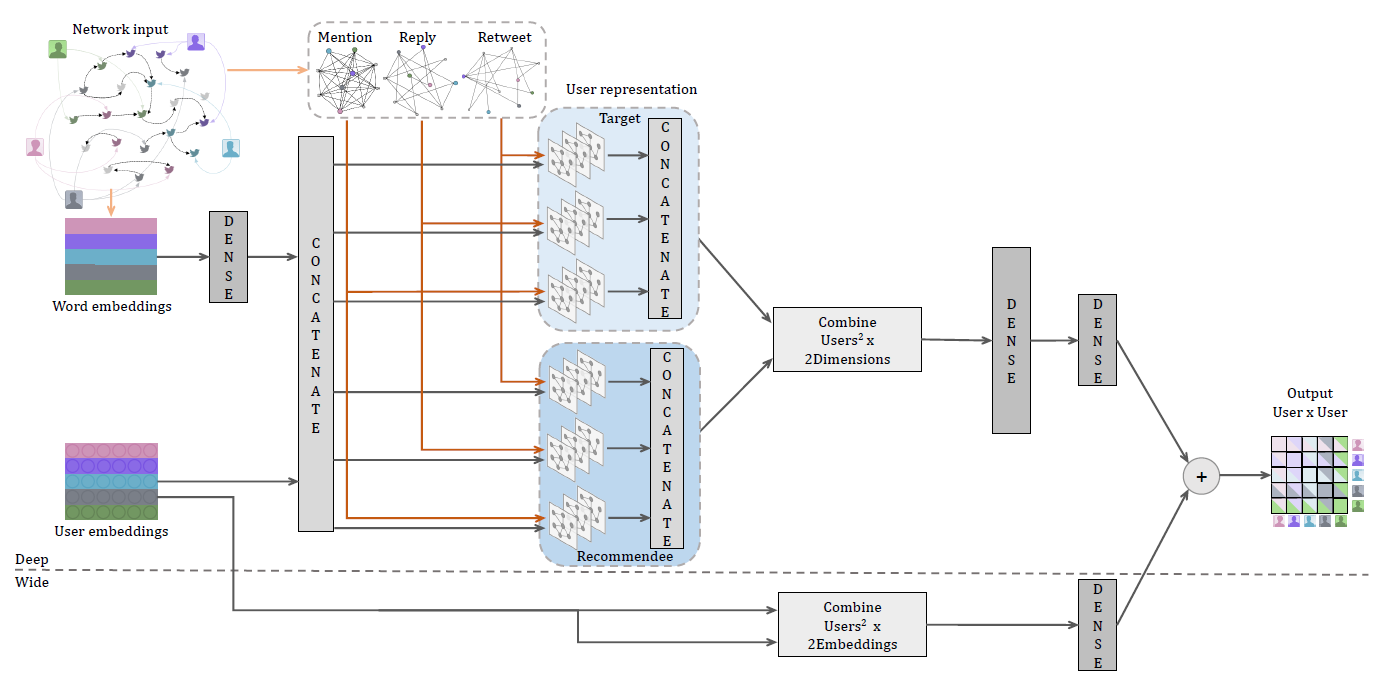
\includegraphics[width=1.0\textwidth]
    {images/FRediECH_architecture.png}
    \caption{Diagram Arsitektur FRediECH
    (diadaptasi dari \textcite{Tommasel2021})}
    \label{fig:arsitektur-FRediECH}
\end{figure}

Pada gambar \ref{fig:arsitektur-FRediECH} terlihat arsitektur FRediECH
yang terinspirasi oleh \textbf{\textit{Graph Convolutional
Network}} (GCN) dan arsitektur \textbf{\textit{Deep \& Wide}}, yang
menggabungkan kesadaran \textit{echo chamber} dan representasi pengguna untuk
menyeimbangkan relevansi, keragaman, dan kebaruan rekomendasi.
\textcite{Tommasel2021} menggunakan GCN paralel untuk mempelajari kontribusi 
spesifik dari jenis interaksi tertentu (seperti \textit{reply}, \textit{mention},
atau \textit{retweet}) terhadap set lengkap hubungan pengguna. Kemudian
luarannya digabungkan untuk menghasilkan representasi pengguna sementara.
(\textit{Loss function}) dalam model ini didefinisikan sebagai jarak antara pengguna dan jumlah interaksi, yang bertujuan untuk memberikan bobot pada interaksi sedemikian rupa sehingga interaksi antara pengguna yang berasal dari
\textit{echo chamber} yang berbeda membawa bobot yang lebih tinggi daripada
interaksi dalam \textit{echo chamber} yang sama. Hal ini akan mempromosikan keragaman
rekomendasi dengan mempelajari struktur komunitas secara implisit
\autocite{Tommasel2021}.

\subsection{Mitigasi Dampak \textit{Echo Chamber} Melalui \textit{Constraint-Based Re-ranking}}
\label{ssec:debiasio_reranking}

Salah satu pendekatan algoritmik terbaru yang secara spesifik menangani dampak rekomendasi terhadap perilaku pengguna adalah kerangka kerja yang diusulkan oleh \textcite{DeBiasio2023}. Penelitian ini membedakan dirinya dari pendekatan diversifikasi umum dengan berfokus pada pelindungan kelompok pengguna sensitif (\textit{sensitive users}) dari paparan berlebih terhadap konten berpengaruh yang dapat memperburuk kondisi perilaku mereka, seperti polarisasi ekstrem atau isolasi sosial.

% \subsubsection{Konsep Pengguna Sensitif dan Item Berpengaruh}
Dalam model \textcite{DeBiasio2023}, masalah \textit{echo chamber} tidak dipandang seragam untuk semua pengguna, melainkan diklasifikasikan berdasarkan kerentanan:
\begin{enumerate}
    \item \textbf{Pengguna Sensitif (\textit{Sensitive Users}):} Kelompok pengguna yang perilakunya rentan dipengaruhi secara negatif oleh pola konsumsi konten yang homogen atau bias.
    \item \textbf{Item Berpengaruh (\textit{Influential Items}):} Kategori konten yang memiliki dampak signifikan terhadap perilaku pengguna sensitif. Item ini dibagi menjadi dua:
    \begin{enumerate}
        \item \textit{Controversial Items}: Item yang jika dikonsumsi berlebihan dapat memperburuk isolasi atau perilaku negatif.
        \item \textit{Favorable Items}: Item yang dapat memberikan dampak positif atau memecah isolasi (\textit{bubble}) jika direkomendasikan dengan proporsi yang cukup.
    \end{enumerate}
\end{enumerate}

Pendekatan ini sangat relevan untuk konteks pembelajaran adaptif karena pengguna sensitif dapat dipetakan sebagai pemelajar yang terisolasi secara akademik, dan \textit{favorable items} sebagai interaksi dengan rekan yang memiliki kompetensi berbeda (heterogen).

% \subsubsection{Algoritma \textit{Re-ranking} Berbasis Batasan}
Untuk memitigasi dampak negatif rekomendasi pada pengguna sensitif tanpa memerlukan pelatihan ulang pada model, \textcite{DeBiasio2023} mengusulkan algoritma \textit{greedy re-ranking}. Algoritma ini bekerja pada tahap pasca-pemrosesan dengan menyusun ulang daftar skor prediksi awal ($\hat{r}_u$) agar memenuhi batasan proporsi item tertentu.

Pada Algoritma \ref{alg:reranking_debiasio} diperlihatkan \textit{pseudocode} dari algoritma \textit{re-ranking} tersebut sebagaimana didefinisikan dalam penelitian aslinya.

\begin{algorithm}[!ht]
\caption{Algoritma Re-ranking (diadaptasi dari \textcite{DeBiasio2023})}
\label{alg:reranking_debiasio}
\begin{algorithmic}[1]
\Require User $u$, Sensitive Set $S$, Predicted Scores $\hat{r}$, Thresholds $\alpha, \beta$, Size $k$
\Ensure Top-$k$ items $Y^*$
\If{$u \notin S$}
    \State \Return \Call{Argsort}{$\hat{r}$}[$0:k$]
\Else
    \State $Y^* \gets \emptyset$
    \State $SortedItems \gets$ \Call{Sort}{$\hat{r}$, 'descending'}
    \For{each item $j \in SortedItems$}
        \If{\Call{Size}{$Y^*$} $< k$}
            \State $CondAlpha \gets ((f_j + \sum_{i \in Y^*} f_i) / k) \geq \alpha$
            \State $CondBeta \gets ((c_j + \sum_{i \in Y^*} c_i) / k) \leq \beta$
            \If{$CondAlpha$ \textbf{and} $CondBeta$}
                \State $Y^* \gets Y^* \cup \{j\}$
            \EndIf
        \Else
            \State \textbf{break}
        \EndIf
    \EndFor
    \State \Return $Y^*$
\EndIf
\end{algorithmic}
\end{algorithm}

Secara matematis, algoritma memastikan bahwa probabilitas terpilihnya
suatu item $y_i$ dalam rekomendasi untuk pengguna sensitif ($s_u=1$) memenuhi
pertidaksamaan berikut,

\begin{align}
    \mathbb{P}(y_i=1 \mid s_u=1, f_i=1) &\geq \alpha \label{eq:constraint_favorable} \\
    \mathbb{P}(y_i=1 \mid s_u=1, c_i=1) &\leq \beta \label{eq:constraint_controversial}
\end{align}
\eqcaption{Batasan Probabilitas Rekomendasi Re-ranking}

dengan:
\begin{itemize}
    \item Persamaan \eqref{eq:constraint_favorable} menetapkan bahwa proporsi
    item \textit{favorable} (yang memecah isolasi) harus lebih besar atau sama
    dengan ambang batas $\alpha$.
    \item Persamaan \eqref{eq:constraint_controversial} menetapkan bahwa proporsi
    item \textit{controversial} (yang memperburuk isolasi) harus lebih kecil
    atau sama dengan ambang batas $\beta$.
\end{itemize}

% \subsubsection{Mekanisme Kerja Algoritma}
Algoritma \textit{re-ranking} ini bekerja dengan menyusun ulang daftar
rekomendasi $\mathcal{Y}_{u,k}$ secara iteratif. Pada setiap langkah penambahan
item ke dalam daftar rekomendasi final, algoritma memeriksa apakah penambahan
item tersebut akan melanggar batasan $\alpha$ atau $\beta$.
\begin{itemize}
    \item Jika daftar rekomendasi saat ini kekurangan item \textit{favorable}
    (di bawah ambang $\alpha$), algoritma akan secara paksa mengambil item
    \textit{favorable} dari daftar cadangan, meskipun skor relevansinya sedikit
    lebih rendah, untuk menggantikan item non-favorable.
    \item Mekanisme ini menjamin terjadinya "eksposur paksa" (\textit{forced
    exposure}) terhadap konten yang beragam, yang merupakan syarat utama untuk
    memecahkan \textit{filter bubble} secara efektif \autocite{DeBiasio2023}.
\end{itemize}

Keunggulan utama pendekatan ini adalah sifatnya yang \textit{model-agnostic} dan
efisien secara komputasi karena menggunakan pendekatan \textit{greedy} pada
tahap \linebreak \textit{post-processing}, sebagaimana dijelaskan secara teknis oleh
\textcite{DeBiasio2023}. Hal ini membuatnya lebih layak diimplementasikan pada
kondisi data terbatas (\textit{cold-start}) dibandingkan metode berbasis
\textit{Deep Learning} yang membutuhkan pelatihan ekstensif.


\section{Pembelajaran Kolaboratif dan CSCL}
\label{sec:collaborative_learning}
Tantangan untuk beralih dari model pedagogi yang berpusat pada pengajar menjadi
berpusat pada pemelajar \autocite{Ryoo2021} sejalan dengan penekanan Strategi Nasional
KA Indonesia pada pentingnya ekosistem kolaboratif \autocite{BPPT2020}. Dalam konteks
pendidikan, filosofi kolaboratif ini sering dimediasi oleh teknologi melalui
\textit{Computer-Supported Collaborative Learning} (CSCL). Bagian ini membahas
prinsip-prinsip dan tantangan dari pendekatan sosial ini, yang menjadi landasan
untuk komponen sosial dari sistem yang diusulkan.

\subsection{Prinsip Pembelajaran Kolaboratif berbasis Teknologi}
\label{ssec:prinsip_cscl}
Pendekatan modern melihat pembelajaran
kolaboratif sebagai proses yang memanfaatkan teknologi untuk mendukung interaksi
sosial. Prinsip-prinsip utamanya adalah sebagai berikut.

\begin{enumerate}
    \item \textbf{Konstruksi Pengetahuan Sosial:} Sistem pembelajaran dapat didasarkan
    pada pendekatan konstruktivis sosial. Dalam model ini, pembelajaran muncul melalui
    interaksi baik dengan rekan yang berpengetahuan (\textit{knowledgeable peers})
    atau dengan sistem AI. Tujuannya adalah untuk mendorong formasi kelompok yang
    heterogen untuk memaksimalkan keragaman kognitif dan mendorong refleksi kritis
    \autocite{Halkiopoulos2024}.

    \item \textbf{Interaksi dalam Komunitas Praktik \textit{(Communities of Practice)}:
    } Teknologi dapat memfasilitasi pembentukan \textit{Communities of Practice} (CoP).
    Sistem \textit{Computer-Supported Collaborative Work} (CSCW) atau proyek berbasis
    tim (\textit{team-based projects}) memungkinkan pemelajar untuk berinteraksi
    dalam ruang tiga dimensi yang sama meskipun secara fisik berada di lokasi yang
    jauh \autocite{Ryoo2021}.
\end{enumerate}

Meskipun prinsip pembentukan kelompok heterogen telah diakui kepentingannya,
tantangan teknis dalam sistem adaptif adalah menentukan standard kuantitatif yang
baku untuk menilai apakah perbedaan kemampuan antarsiswa sudah cukup signifikan
untuk disebut heterogen.

\subsection{Pengukuran Heterogenitas Kelompok dan \textit{Effect Size}}

Dalam ranah ilmu perilaku dan pendidikan, pengukuran perbedaan antara dua \linebreak kelompok
atau individu tidak cukup hanya dengan melihat selisih nilai mentah (\textit{raw
score differences}), karena nilai tersebut sangat bergantung pada satuan skala
yang digunakan. Untuk mengatasi hal ini, \textcite{Cohen1988} memperkenalkan
konsep \textit{Effect Size} (ES) sebagai indeks standard yang independen dari
satuan pengukuran asal. Salah satu indeks ES yang paling fundamental dan banyak
digunakan untuk membandingkan dua rata-rata adalah \textit{Cohen's d}. Secara
konseptual, \textit{Cohen's d} didefinisikan sebagai selisih antara dua rata-rata
populasi ($m_A - m_B$) yang dibagi dengan standar deviasi populasi ($\sigma$).
Rasio ini merepresentasikan jarak antara dua rata-rata dalam satuan unit
variabilitas standard, memberikan ukuran murni mengenai seberapa jauh dua
distribusi nilai terpisah satu sama lain.

Dalam praktiknya, ketika parameter populasi tidak diketahui, nilai $d$ diestimasi
\linebreak menggunakan statistik sampel. \textcite{Cohen1988} merumuskan penghitungan $d$
untuk dua sampel independen dengan menggunakan \textit{pooled standard deviation}
($\sigma_{pooled}$) sebagai penyebut, yang merupakan rata-rata akar kuadrat dari
varians kedua kelompok. Rumus formal untuk menghitung jarak atau indeks perbedaan
ini dinyatakan sebagai berikut,

\begin{align}
    d &= \frac{| \bar{x}_A - \bar{x}_B |}{\sigma_{pooled}} \label{eq:cohen_d_basic} \\
    \sigma_{pooled} &= \sqrt{\frac{(n_A-1)s_A^2 + (n_B-1)s_B^2}{n_A + n_B - 2}} \label{eq:sigma_pooled}
\end{align}
\eqcaption{Persamaan Cohen's d}

dengan $\bar{x}_A$ dan $\bar{x}_B$ adalah nilai rata-rata (atau skor kemampuan
individu) dari dua entitas yang dibandingkan, $s_A^2$ dan $s_B^2$ adalah varians
masing-masing, serta $n_A$ dan $n_B$ adalah ukuran sampel. Jika diaplikasikan pada
perbandingan antarindividu (dengan $n=1$), penyebut dapat disederhanakan menjadi
standar deviasi gabungan dari populasi referensi atau data historis sistem. Nilai
$d$ yang dihasilkan adalah nilai skalar tak berdimensi yang memungkinkan
perbandingan yang adil meskipun diterapkan lintas konteks.

Untuk memberikan makna interpretatif pada nilai numerik $d$, \textcite{Cohen1988} menetapkan standard konvensi yang menjadi rujukan universal dalam analisis kuantitatif. Konvensi ini dirancang untuk memetakan besaran statistik ke dalam dampak kualitatif yang dapat diamati di dunia nyata.
\begin{enumerate}
    \item \textbf{Efek Kecil ($d = 0.2$):} Perbedaan yang nyata namun sulit dideteksi tanpa analisis statistik yang cermat.
    \item \textbf{Efek Sedang ($d = 0.5$):} Perbedaan yang cukup besar untuk dapat dilihat oleh mata telanjang pengamat yang berpengalaman (\textit{visible to the naked eye}).
    \item \textbf{Efek Besar ($d = 0.8$):} Perbedaan yang sangat mencolok, setara dengan perbedaan tinggi badan antara remaja usia 13 dan 18 tahun.
\end{enumerate}

Standard operasional ini memberikan landasan teoretis untuk menetapkan ambang batas (\textit{threshold}) penentuan apakah dua entitas (atau kelompok) dapat dikategorikan berbeda secara signifikan (heterogen).

\subsection{Aktivitas Pembelajaran Sosial dan Dampaknya}
\label{ssec:aktivitas_pembelajaran_sosial}
Selain prinsip-prinsip umum yang telah dibahas pada Subbab
\ref{ssec:prinsip_cscl}, penting untuk mengidentifikasi bentuk-bentuk aktivitas pembelajaran sosial spesifik yang telah terbukti memiliki dampak
positif terhadap hasil belajar. Aktivitas-aktivitas inilah yang menjadi kandidat
utama untuk diintegrasikan dan dinilai dalam sebuah sistem adaptif.

\begin{enumerate}
    % \subsubsection{Penilaian Sejawat (\textit{Peer Assessment})}
    % \label{sssec:peer_assessment}
    \item \textbf{Penilaian sejawat (\textit{Peer Assessment}):}
    Penilaian sejawat adalah aktivitas pendidikan yang mengajak
    pemelajar saling menilai pekerjaan satu sama lain, artinya dalam
    penilaian ini penilai (\textit{assessor}) dan yang dinilai
    (\textit{assessed}) memiliki kedudukan yang sama
    \autocite{Ihichr2024}.
    
    Evaluasi terhadap kinerja penilai dalam
    \textit{peer assessment} tidak cukup hanya didasarkan
    pada akurasi skor (\textit{rating accuracy}), tetapi
    juga harus meninjau kualitas umpan balik tekstual yang
    diberikan secara terukur. \textcite{Kerman2024}
    mengembangkan skema pengodean yang membagi fitur umpan
    balik ke dalam tiga elemen utama: (1) \textit{Affective}
    (afektif), yang mencakup emosi positif seperti pujian
    atau emosi negatif, (2) \textit{Cognitive} (kognitif),
    yang terdiri dari deskripsi ringkasan (\textit{description}),
    identifikasi masalah (\textit{identification}), dan
    justifikasi masalah (\textit{justification}),
    serta (3) \textit{Constructive} (konstruktif)
    yang mencakup rekomendasi solusi.
    
    Keunggulan dari pendekatan ini adalah kemampuannya
    untuk menguantifikasi kualitas umpan balik secara
    granular. Dalam rubrik yang diusulkan
    \textcite{Kerman2024}, setiap fitur dinilai dengan
    skor dari nol (kualitas buruk) hingga dua (kualitas baik).
    Sebagai contoh, pada dimensi \textit{Constructive},
    skor 0 diberikan jika tidak ada rekomendasi, skor 1 jika
    hanya ada rekomendasi tanpa rencana aksi, dan skor 2 jika
    terdapat rekomendasi beserta rencana aksi (\textit{action
    plans}) untuk perbaikan lebih lanjut. Penjumlahan poin-poin
    ini merepresentasikan skor keseluruhan kualitas umpan
    balik yang dihasilkan oleh pemelajar.
    
    Pentingnya menekankan aspek kognitif dan konstruktif
    didukung oleh temuan empiris bahwa fitur-fitur inilah
    yang menjadi prediktor kesuksesan revisi tugas.
    \textcite{Kerman2024} menemukan bahwa pemelajar yang sukses
    cenderung menerima umpan
    balik yang berfokus pada \textit{identification}
    (identifikasi masalah), sedangkan umpan balik yang murni
    afektif atau sekadar deskriptif lebih banyak
    diterima oleh pemelajar yang kurang berhasil. Hal ini
    menunjukkan bahwa untuk meningkatkan kompetensi, sistem
    harus mendorong pemelajar untuk memberikan komentar yang
    tidak hanya menyentuh aspek emosional, tetapi memberikan
    identifikasi masalah dan solusi konkret.
    
    % \subsubsection{Pembelajaran Berbasis Proyek (\textit{Project-Based Learning})}
    % \label{sssec:pbl}
    \item \textbf{Pembelajaran Berbasis Proyek (\textit{Project-Based Learning}):} Pembelajaran berbasis proyek (PBL) adalah model pembelajaran yang
    berpusat pada pemelajar, dengan tujuan menghasilkan sebuah karya proyek yang memecahkan masalah dunia nyata \autocite{Zhang2023}. Berbeda
    dengan pembelajaran tradisional, PBL menempatkan pemelajar dalam peran aktif untuk
    berkolaborasi, mengintegrasikan berbagai disiplin ilmu, dan menerapkan pengetahuan
    \autocite{Ryoo2021}. Sebuah metaanalisis oleh \textcite{Zhang2023} terhadap 66 studi eksperimental
    menemukan bahwa PBL secara signifikan meningkatkan hasil belajar pemelajar
    dibandingkan dengan model pengajaran tradisional. Dampak
    positif ini terukur pada tiga dimensi luaran pembelajaran, yaitu
    pencapaian akademik, sikap afektif, dan keterampilan berpikir \autocite{Zhang2023}.

    % \subsubsection{Pendampingan Sejawat (\textit{Peer Mentoring})}
    % \label{sssec:peer_mentoring}
    \item \textbf{Pendampingan Sejawat (\textit{Peer Mentoring}):} \textit{Peer mentoring} adalah mekanisme bimbingan individual
    yang diberikan oleh pemelajar senior untuk membantu pemelajar lain \autocite{Le2024}.
    Aktivitas ini dirancang untuk membantu pemelajar baru (\textit{mentee}) dalam
    menavigasi tantangan transisi ke pendidikan tinggi, baik secara akademik maupun
    sosial. Sebuah tinjauan sistematis baru-baru ini yang mencakup 27 studi empiris
    mengidentifikasi empat kategori manfaat fundamental dari \textit{peer mentoring}
    bagi \textit{mentee}. Manfaat tersebut adalah: (1) peningkatan kinerja akademik
    (\textit{academic performance}), (2) peningkatan retensi
    (\textit{retention rates}) atau persistensi, (3) peningkatan kesejahteraan
    emosional dan psikologis (\textit{emotional and psychological wellbeing}), dan
    (4) kesatuan sosial (\textit{social integration}) yang lebih baik di
    lingkungan kampus \autocite{Le2024}.
    
    % \subsubsection{Sesi Diskusi Terbuka}
    % \label{sssec:open_discussion}
    \item \textbf{Sesi Diskusi Terbuka:} Interaksi sosial langsung melalui diskusi juga terbukti berdampak pada hasil
    belajar. Sebuah studi oleh \textcite{DaifAllah2016} menginvestigasi dampak dari
    Sesi Diskusi Terbuka (\textit{Open Discussion Sessions}) yang diadakan sebagai
    kegiatan ekstrakurikuler untuk meningkatkan kemampuan komunikasi lisan pemelajar.
    Hasil studi menunjukkan adanya perkembangan signifikan dalam kemampuan berbicara
    pemelajar. Keberhasilan ini adalah efek dari faktor-faktor kunci dalam desain aktivitas tersebut, yaitu penyediaan lingkungan
    belajar yang santai dan bebas rasa khawatir (\textit{relaxed learning environment
    void of worry}) serta keterlibatan aktif dengan situasi komunikatif nyata
    (\textit{active involvement with real communicative situations})
    \autocite{DaifAllah2016}.

    % \subsubsection{Bermain Peran (\textit{Role-Playing})}
    % \label{sssec:role_play}
    \item \textbf{Bermain Peran (\textit{Role-Playing}):} metode bermain peran adalah metode pengajaran simulasi situasional. Pada
    metode ini, pemelajar diminta untuk mengambil peran spesifik untuk mensimulasikan
    skenario dunia nyata. Pendekatan ini memindahkan fokus dari
    pengetahuan teoretis ke penerapan praktis dan pengembangan keterampilan.
    Sebuah metaanalisis yang mensintesis 12 artikel menemukan
    bahwa pengajaran menggunakan metode bermain peran memiliki efek positif yang
    signifikan (\textit{ES}=0.818) pada pemelajar dibandingkan dengan kelompok kontrol
    yang menggunakan pengajaran tradisional. Secara khusus,
    ditemukan bahwa metode bermain peran memiliki dampak paling signifikan pada
    peningkatan keterampilan pemelajar \autocite{Fu2025}.
\end{enumerate}

\subsection{Tantangan dalam Menilai Kolaborasi}
\label{ssec:tantangan_menilai_kolaborasi}
Meskipun manfaat pedagogisnya jelas, menilai pembelajaran kolaboratif secara
adil menghadirkan tantangan yang signifikan. Masalah utamanya adalah bagaimana
mengukur kontribusi individu secara akurat di dalam kelompok.

Salah satu tantangan utama adalah metode penilaian kinerja dalam kelompok
yang tujuannya adalah pemecahan masalah secara kreatif sehingga tidak fokus mengukur bagaimana setiap orang berkontribusi pada kelompok mereka dan bagaimana efek dari kontribusi individual tersebut terhadap kuantitas maupun kualitas hasil akhir \autocite{Ryoo2021}. Untuk mengatasi ini, \textit{peer assessment} (penilaian sejawat) sering digunakan. Ini dijelaskan sebagai aktivitas pendidikan yang menghadirkan penilai dan yang dinilai dalam status yang sama,
dan masing-masing menilai hasil dan kualitas belajar satu sama lain
\autocite{Ihichr2024}. Studi oleh \textcite{Ihichr2024} mencatat bahwa pemelajar mendapat lebih banyak manfaat dari bertindak sebagai penilai daripada hanya dinilai.

Tantangan kedua, yang secara khusus relevan dengan penelitian ini, adalah risiko (\textit{overpersonalization}) dalam sistem adaptif
berbasis AI. Sistem yang terlalu fokus pada optimasi jalur belajar individu dapat
menyebabkan pemelajar yang mendapat manfaat dari pembelajaran
bersama (\textit{shared learning}) akan terasingkan dalam sistem.
\textit{Overpersonalization} ini dapat menjadi penghalang ketika pemelajar seharusnya mampu memperoleh manfaat dari keberagaman perspektif dalam komunitas pembelajarannya. Oleh karena itu,
sistem asesmen adaptif modern harus mampu menyeimbangkan antara personalisasi
individu dengan fasilitasi interaksi sosial \autocite{Halkiopoulos2024}.

% \subsection{Metode Pembobotan Penilaian Terintegrasi}
% \label{ssec:pembobotan_terintegrasi}
Terakhir, dalam mengintegrasikan skor kemahiran personal dan performa sosial, penentuan bobot yang adil juga menjadi tantangan tersendiri. Penelitian oleh \textcite{Demetroulis2024} mengusulkan skema pembobotan yang memberikan porsi kontribusi individu sebesar 80\%, sementara performa kelompok secara keseluruhan diberikan porsi 20\%. Rasio 80:20 ini bertujuan untuk menghargai input kognitif dan strategis individu dalam tim yang mungkin tidak selalu terlihat dalam hasil akhir, namun tetap memberikan insentif terhadap keberhasilan kerja sama kelompok. Fokus utama dari pembobotan ini adalah pada proses kolaboratif individu alih-alih hanya mengandalkan hasil akhir kolektif (\textit{collaborative outcome}).

\section{Upaya Integrasi Penilaian Personal dalam Lingkungan Kolaboratif yang Sudah Ada Saat Ini}
\label{sec:upaya_integrasi}

Tinjauan literatur menunjukkan bahwa sebagian besar penelitian dan
implementasi sistem pembelajaran adaptif hingga saat ini berfokus secara
dominan pada pemelajar individu. Sistem \textit{e-learning} yang ada, sering kali
dirancang untuk mengadaptasi konten dan urutan penyampaiannya sesuai dengan
kemampuan pemelajar secara individual \autocite{Halkiopoulos2024}. Fokus pada
personalisasi ini terlihat jelas dalam model-model asesmen seperti
\textit{Item Response Theory} (IRT), \textit{Bayesian Knowledge Tracing} (BKT),
dan \textit{Deep Knowledge Tracing} (DKT), yang pada intinya memodelkan keadaan
pengetahuan laten seorang pemelajar tunggal \autocite{Minn2022}.

Meskipun personalisasi ini ada manfaatnya,
\textcite{Halkiopoulos2024} memperingatkan adanya risiko
(\textit{overpersonalization}). Pendekatan yang terlalu terindividualisasi dapat menciptakan situasi yang menyebabkan pemelajar yang seharusnya bisa mendapat manfaat dari pembelajaran bersama (\textit{shared learning}) malah terasingkan sehingga menghambat perolehan manfaat dari keberagaman perspektif dalam komunitas pembelajaran.

Beberapa penelitian telah mengeksplorasi penggunaan AI dalam konteks
kolaboratif, tetapi sering kali terpisah dari siklus asesmen adaptif
inti. Sebagai contoh, \textcite{Nalli2022} menggunakan teknik \textit{clustering} untuk membantu pengajar dalam pembentukan kelompok heterogen. Dalam studi ini,
AI digunakan sebagai alat bantu persiapan (\textit{setup tool}) yang efektif
untuk formasi kelompok, bukan sebagai mesin yang secara dinamis menilai kolaborasi
atau mengadaptasi konten secara \textit{near real-time} berdasarkan interaksi kelompok.

Upaya yang lebih dekat dengan integrasi ideal dengan sistem asesmen adaptif adalah
\textit{Open Social Student Modeling} (OSSM) yang diperkenalkan oleh
\textcite{Brusilovsky2016}.

\begin{figure}[!ht] 
    \centering
    \captionsetup{justification=centering}
    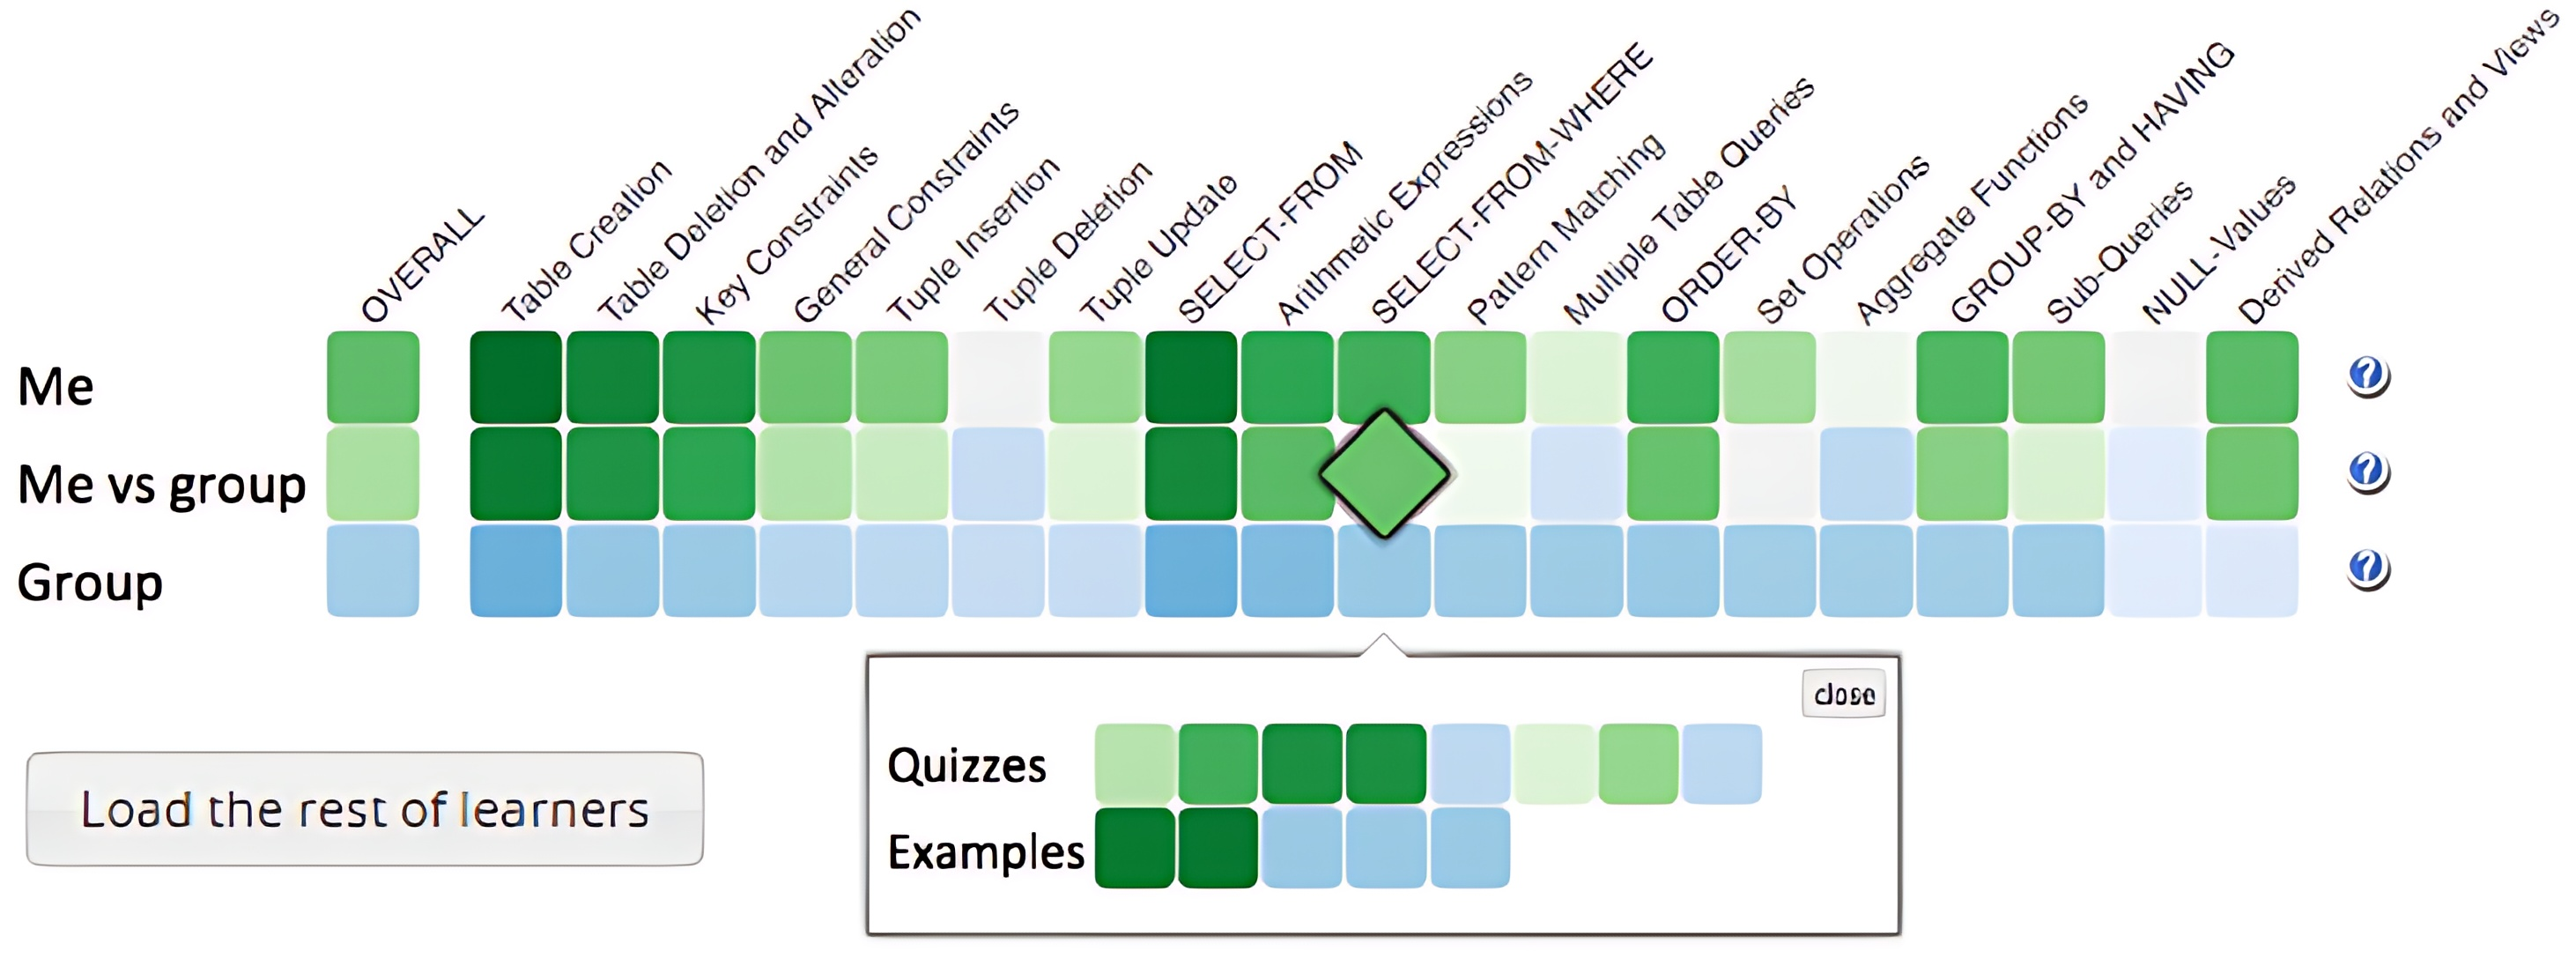
\includegraphics[width=1.0\textwidth]
    {images/brusilovsky_fig1a_processed.jpg}
    \caption{Model Konseptual Antarmuka Pembelajaran
    Sosial (OSSM) (diadaptasi dari \textcite{Brusilovsky2016})}
    \label{fig:model-konseptual-sosial}
\end{figure}

Dalam implementasinya pada sistem MasteryGrids,
OSSM melengkapi aspek kognitif dengan aspek sosial melalui antarmuka yang
menampilkan visualisasi perbandingan kinerja \textit{Me vs group} (Saya vs grup). Meskipun studi mereka menemukan bahwa fitur
eksplorasi sosial ini dapat meningkatkan pembelajaran, terutama bagi pemelajar dengan pengetahuan awal rendah, pendekatan ini pada hakekatnya bersifat visualisasi. \textcite{Brusilovsky2016} menempatkan aspek sosial sebagai \textit{output} untuk memotivasi pemelajar.

% , namun tidak merinci bagaimana data perbandingan sosial ini diintegrasikan kembali sebagai \textit{input} ke dalam algoritma asesmen inti (seperti \textit{Elo rating} atau BKT) untuk
% mengubah perhitungan kemahiran individu secara dinamis atau merekomendasikan
% intervensi kolaboratif.

\section{Strategi Desain Asesmen Formatif Daring}
\label{sec:strategi_asesmen_formatif}

Implementasi asesmen adaptif dalam lingkungan digital memerlukan strategi desain instrumen yang tidak hanya mengandalkan algoritma, tetapi juga mempertimbangkan mekanisme interaksi pemelajar dengan soal untuk mendukung tujuan pembelajaran formatif. Bagian ini membahas landasan teoretis mengenai implementasi pembelajaran daring yang mengintegrasikan fitur percobaan berulang dan sistem umpan balik otomatis sebagai upaya untuk meningkatkan pemahaman konsep secara mandiri.

\subsection{Ukuran Bank Soal dalam Implementasi Asesmen Adaptif}
\label{ssec:ukuran_bank_soal}

Penelitian oleh \textcite{Hadi2022} dilatarbelakangi oleh permasalahan metode pengujian tradisional di sekolah vokasi yang sering kali gagal dalam membedakan kemampuan awal pemelajar secara akurat. Untuk mengatasi masalah tersebut, studi tersebut bertujuan untuk mengembangkan dan menguji kelayakan alat asesmen kelas menggunakan \textit{Computerized Adaptive Test} (CAT) berbasis \textit{Learning Management System} (LMS). Penelitian ini difokuskan secara spesifik pada program studi Teknik Instalasi Tenaga Listrik untuk memberikan penilaian yang lebih representatif bagi pemelajar. Metodologi yang digunakan dalam penelitian ini adalah pendekatan \textit{Research and Development} (R\&D) yang mencakup konstruksi skala dan pengumpulan bank soal. Proses pengembangan tersebut melibatkan pengumpulan data dari responden ahli serta pemelajar untuk memastikan validitas instrumen yang dibangun.

Instrumen yang berhasil dikembangkan dalam penelitian \textcite{Hadi2022} tersebut terdiri dari 60 butir soal pilihan ganda yang diintegrasikan ke dalam modul kuis adaptif pada LMS Moodle. Analisis butir soal dilakukan menggunakan Model Rasch dan Teori Tes Klasik (\textit{Classical Test Theory}) untuk mengevaluasi sifat psikometrik dari bank soal tersebut. Hasil pengujian menunjukkan bahwa instrumen ini memiliki tingkat validitas dan reliabilitas yang sangat tinggi dengan nilai koefisien Alpha mencapai 0,934. Studi tersebut menyimpulkan bahwa pengujian adaptif berbasis LMS ini mampu memberikan pengukuran yang lebih presisi dengan jumlah pertanyaan yang lebih sedikit dibandingkan tes konvensional. Dengan demikian, penelitian ini membuktikan bahwa integrasi CAT ke dalam LMS sekolah sangat layak diterapkan untuk mendukung pengambilan keputusan instruksional dan pembelajaran terpersonalisasi.

\subsection{Mekanisme Percobaan Berulang (\textit{Multiple Attempts})}
\label{ssec:mekanisme_percobaan_berulang}

Penggunaan kuis daring dengan fitur percobaan berulang (\textit{multiple attempts}) merupakan bagian dari asesmen formatif yang bertujuan untuk meningkatkan proses berpikir dan pemahaman konsep pemelajar terhadap materi pembelajaran. Menurut \textcite{Mendoza2022}, pemberian kesempatan bagi pemelajar untuk mengerjakan soal kuis lebih dari satu kali memungkinkan mereka untuk mengenali celah dalam pemahaman kurikulum serta memantau progres belajar secara mandiri selama proses berlangsung. Hasil penelitian menunjukkan bahwa rata-rata nilai pada kuis daring dengan percobaan berulang terbukti menjadi prediktor yang signifikan terhadap pencapaian nilai pemelajar pada ujian akhir. Selain itu, pemelajar cenderung menunjukkan peningkatan skor yang signifikan dan waktu pengerjaan yang lebih singkat pada percobaan terakhir dibandingkan dengan percobaan pertama mereka setelah mendapatkan intervensi. Implementasi mekanisme ini juga terbukti memotivasi pemelajar untuk menyelesaikan tugas persiapan, meningkatkan partisipasi dalam diskusi kelas, dan secara umum meningkatkan kinerja akademik pada ujian sumatif.

Dalam konteks jumlah upaya yang diberikan, penggunaan batasan tiga kali percobaan (\textit{three attempts}) teridentifikasi memiliki dampak positif yang signifikan terhadap peningkatan nilai kuis daring pemelajar secara konsisten. \textcite{Mendoza2022} menjelaskan bahwa pada percobaan kedua dan ketiga, pemelajar diwajibkan untuk menjawab kembali seluruh butir soal guna memperbaiki kesalahan dari percobaan sebelumnya sekaligus memastikan penguasaan konsep pada jawaban yang sudah benar. Persyaratan untuk menunjukkan solusi lengkap pada setiap percobaan bertujuan untuk mencegah pemelajar melakukan penebakan jawaban secara sembarangan (\textit{guessing}) dan mendorong mereka untuk benar-benar belajar dari umpan balik yang diberikan sistem. Analisis kuantitatif melalui uji ANOVA menunjukkan bahwa terjadi peningkatan rerata nilai yang konsisten di seluruh instrumen kuis yang diujikan dalam kerangka tiga kali percobaan tersebut. Oleh karena itu, batasan tiga kali upaya ini dipandang mampu memberikan ruang yang cukup bagi pemelajar untuk melakukan evaluasi diri dan melakukan penyuntingan terhadap pekerjaan mereka sendiri (\textit{self-edit}).

\subsection{Sistem Umpan Balik Otomatis (\textit{Automated Feedback System})}
\label{ssec:sistem_umpan_balik_otomatis}

Integrasi sistem umpan balik otomatis dalam kuis daring merupakan elemen krusial untuk mengatasi keterbatasan pengajar dalam memberikan koreksi secara instan dan berkelanjutan pada kelas dengan jumlah pemelajar yang besar. \textcite{Mendoza2022} menyatakan bahwa umpan balik yang diberikan secara tepat waktu, spesifik, dan berkelanjutan sangat penting untuk memperbaiki kesalahan serta kekeliruan pemelajar selama proses asesmen berlangsung agar tidak terulang kembali. Penggunaan teknologi digital dalam penyampaian umpan balik berpotensi meningkatkan kualitas respons serta menghemat waktu pemeriksaan bagi pengajar dibandingkan dengan metode tertulis tradisional. Umpan balik yang efektif harus memiliki karakteristik yang mudah dipahami, selektif, spesifik, tepat waktu, kontekstual, dan berorientasi ke depan agar dapat memicu tindakan perbaikan lebih lanjut dari sisi pemelajar. Selain itu, umpan balik elektronik dapat mengurangi hambatan logistik sambil tetap mempertahankan fitur-fitur terbaik dari umpan balik tradisional yang bersifat jelas dan komprehensif bagi penerimanya.

Dampak dari sistem umpan balik otomatis ini tercermin pada persepsi positif pemelajar yang menganggapnya sebagai panduan yang berguna dalam memahami materi pembelajaran meskipun tanpa kehadiran fisik pengajar secara langsung. Berdasarkan temuan \textcite{Mendoza2022}, mayoritas pemelajar merasa terbantu dalam mengidentifikasi aspek materi yang belum dikuasai serta keterampilan spesifik yang perlu mereka tingkatkan melalui pesan koreksi yang muncul setelah setiap jawaban diberikan. Umpan balik yang dirancang dengan mempertimbangkan alasan masuk akal dari pilihan jawaban salah (\textit{plausible distractors}) memungkinkan pemelajar untuk melakukan komputasi ulang dan mengingat kembali konsep yang telah diajarkan sebelumnya. Penting untuk dicatat bahwa umpan balik dalam sistem ini idealnya bersifat menyarankan (\textit{suggestive}) dan bukan memerintah (\textit{prescriptive}), sehingga pemelajar tetap memiliki otonomi dan kebebasan dalam menentukan cara pemecahan masalah sesuai preferensi mereka sendiri. Dengan demikian, ketersediaan umpan balik yang instan bersamaan dengan fitur percobaan berulang menciptakan ruang interaksi yang bermakna antara pemelajar dan sistem untuk meminimalkan stagnasi pembelajaran.

\subsection{Evaluasi Kebenaran Kueri SQL}
\label{ssec:evaluasi_kueri_sql}
SQL (\textit{Structured Query Language}) secara teoretis merupakan bahasa deklaratif yang didasarkan pada kalkulus relasional, di mana kueri mendefinisikan informasi apa yang ingin diambil tanpa merinci alur prosedural untuk memperolehnya \autocite{Silberschatz2019}. Akibatnya, satu pernyataan tujuan informasi yang sama dapat diekspresikan melalui berbagai struktur sintaksis yang berbeda. 

Menurut \textcite{Silberschatz2019}, proses evaluasi kueri dimulai dari penerjemahan kueri deklaratif ke dalam representasi prosedural berupa ekspresi aljabar relasional, yang kemudian dioptimalkan menjadi rencana evaluasi kueri (\textit{query evaluation plan}). Dalam optimasi kueri, terdapat berbagai alternatif rencana evaluasi yang setara secara semantik (\textit{semantic equivalence}), yaitu menghasilkan luaran yang identik untuk setiap instans basis data yang valid. Ekuivalensi ini dianalisis menggunakan aturan ekuivalensi aljabar relasional untuk merestrukturisasi ekspresi tanpa mengubah makna semantiknya. Namun, secara teoretis, menentukan ekuivalensi semantik antara dua ekspresi relasional sembarang merupakan permasalahan komputasi yang sangat kompleks dan tergolong sebagai masalah tidak terputuskan (\textit{undecidable}) pada kasus umum, serta termasuk dalam kategori NP-Hard untuk subset kueri konjungtif. Oleh karena itu, kajian teoretis optimasi kueri berfokus pada penggunaan heuristik dan aturan transformasi lokal untuk menjelajahi ruang pencarian rencana evaluasi yang setara secara efisien.

\section{Metodologi Evaluasi Purwarupa Sistem Pembelajaran}
\label{sec:metodologi_evaluasi}

\subsection{Pengukuran Efektivitas dengan \textit{Normalized Learning Gain} (NLG)}
\label{ssec:nlg}
Dalam ranah penelitian pendidikan fisika dan teknologi pembelajaran, pengukuran
efektivitas intervensi instruksional sering kali menghadapi tantangan bias yang
disebabkan oleh perbedaan tingkat pengetahuan awal pemelajar. Untuk mengatasi hal
ini, Richard Hake memperkenalkan konsep \textit{average normalized gain} ($g$)
sebagai metrik standard. Secara teoretis, \textit{normalized gain} didefinisikan
sebagai rasio antara peningkatan skor aktual yang dicapai (\textit{actual gain})
terhadap peningkatan skor maksimum yang mungkin dicapai (\textit{maximum possible
gain}). Penggunaan metrik ini bertujuan untuk memisahkan efek pembelajaran dari
pengaruh skor \textit{pre-test} sehingga memungkinkan perbandingan yang objektif
antara populasi pemelajar yang memiliki latar belakang kemampuan yang heterogen
\autocite{Nissen2018}.

Secara matematis, perhitungan \textit{normalized gain} untuk rata-rata kelas
atau individu pada umumnya dinyatakan dalam persamaan berikut:

\begin{align}
    g &= \frac{\text{post} - \text{pre}}{\text{maksimum} - \text{pre}} \label{eq:normalized_gain_formula}
\end{align}
\eqcaption{Persamaan Normalized Learning Gain}

dengan $\text{pre}$ merepresentasikan skor pada tes awal sebelum
instruksi diberikan, $\text{post}$ adalah skor pada tes akhir, dan $\text{maksimum}$ adalah batas atas skor yang dapat dicapai. Pada sistem yang menggunakan pengukuran skala kontinu seperti \textit{Elo rating}, nilai maksimum ini disesuaikan dengan ambang batas \textit{Elo} tertinggi (baik secara teoretis maupun empiris).
\textcite{Coletta2020} menegaskan bahwa metrik ini memiliki keunggulan teoretis
dibandingkan perhitungan selisih skor mentah atau \textit{effect size} standard
(seperti Cohen's $d$), terutama dalam menangani distribusi data yang mengalami
\textit{floor effect} atau \textit{ceiling effect} ekstrem, sebuah efek yang
mengakibatkan pemelajar dengan
skor awal tinggi memiliki ruang peningkatan yang lebih sempit dibandingkan pemelajar
dengan skor rendah.

Sebagai standard interpretasi efektivitas yang berlaku umum dalam literatur, Hake
menetapkan kriteria ambang batas untuk mengkategorikan tingkat keberhasilan
pembelajaran. Nilai $g$ diklasifikasikan ke dalam tiga kategori:

\begin{enumerate}[1.]
    \item \textbf{Rendah} (\textit{Low-g}) jika $g < 0{,}3$; 
    \item \textbf{Sedang}
    (\textit{Medium-g}) jika $0{,}3 \leq g < 0{,}7$; dan 
    \item \textbf{Tinggi}
    (\textit{High-g}) jika $g \geq 0{,}7$.
\end{enumerate}

Klasifikasi ini menyediakan kerangka kerja komparatif yang konsisten bagi para peneliti untuk mengevaluasi apakah sebuah
metode pedagogis mampu menghasilkan peningkatan pemahaman konsep yang substansial
terlepas dari kesulitan materi yang diajarkan \autocite{Coletta2020}.

\subsection{Penentuan Ukuran Sampel dalam Studi Pilot}
\label{ssec:ukuran_sampel}
Dalam pengujian purwarupa sistem yang bersifat eksploratif, metodologi yang digunakan sering kali dikategorikan sebagai studi pilot atau penelitian pendahuluan (\textit{preliminary research}). Menurut \textcite{Sukserm2024}, penentuan ukuran sampel yang tepat sangat krusial untuk memastikan bahwa hasil pengujian dapat memberikan gambaran valid mengenai kelayakan instrumen dan desain penelitian.

Berdasarkan tinjauan yang dilakukan oleh \textcite{Sukserm2024}, para peneliti merekomendasikan rentang sampel antara 10 hingga 30 partisipan untuk studi pilot. Secara khusus, Johanson dan Brooks (2010) (sebagaimana dikutip dalam \textcite{Sukserm2024}) menyatakan bahwa jumlah minimal 10 partisipan sudah cukup memadai untuk mengidentifikasi masalah utama dalam desain dan memvalidasi instrumen sebelum melangkah ke studi skala besar. Dengan demikian, penggunaan angka 10 sebagai batas minimum jumlah partisipan per kelompok dalam penelitian ini dianggap sah secara metodologis untuk mengevaluasi fungsionalitas purwarupa.

